\documentclass{fast-nuces-bs}

% -------------------------
% PACKAGE IMPORTS
% Loads layout, figures, tables, algorithms, and hyperlink support.
\usepackage{blindtext}
\usepackage{tikz}
\usepackage{mathptmx}
\usepackage[T1]{fontenc}
\usepackage{lipsum}
\usepackage{sectsty}
\usepackage{titlesec}
\usepackage{graphicx}
\usepackage{float}
\usepackage{array}
\usepackage{booktabs}
\usepackage{geometry}
\usepackage{adjustbox}
\usepackage{pdflscape}
\usepackage{caption}
\usepackage{subcaption}
\usepackage{tabularx}
\usepackage{placeins}   % \FloatBarrier
\usepackage{needspace}
\usepackage{rotating}   % sidewaysfigure if needed
\usepackage{hyperref}
\usepackage{url}         % For url commands
\usepackage{amsmath}    % For mathematical equations
\usepackage{algorithm}
\usepackage{algpseudocode}
\geometry{margin=1in}
\titlespacing*{\section}{0pt}{16pt}{8pt}
\titlespacing*{\subsection}{0pt}{12pt}{6pt}

% -------------------------
% LAYOUT TUNING
% Adjusts heading and float spacing for cleaner page flow.
\setlength{\intextsep}{8pt}
\setlength{\textfloatsep}{10pt}
\setlength{\floatsep}{8pt}
\Urlmuskip=0mu plus 2mu\relax
\emergencystretch=2em

% Prevent double blank pages between chapters.
\let\cleardoublepage\clearpage
\flushbottom

% -------------------------
% DOCUMENT METADATA
% Defines title-page and degree information.
\department{Department of Software Engineering}
\faculty{Computer Science}
\degreeyear{2026}
\degreemonth{April}
\degreename{Bachelor of Science in Software Engineering}
\campuscity{Peshawar}
\authorone{Alishba Tariq }{22P-9112 }
\authortwo{Muhammad Hasnain Saleem}{22P-9123}
\authorthree{Kashan Saeed}{22P-9128}
\supervisor{Dr. Nouman Azam}
\sessionduration{2022--2026}
\directorname{Dr. Omar Usman, Director of the Campus}
\hodname{Dr. Qasm Jan}
\fypcoordinatorname{Mr. Riaz Nawab}
\title{AutoReturn \\ \large An Agentic Unified Intelligent Multi-Platform Communication System}
\certificatetitle{AutoReturn: An Agentic Unified Intelligent Multi-Platform Communication System}

% -------------------------
% FRONT MATTER
% Includes acknowledgements and abstract.
\begin{document}

\begin{acknowledgements}
We would like to express our deepest gratitude to our supervisor, \textbf{Dr. Nouman Azam}, for his continuous guidance, motivation, and valuable knowledge throughout the development of our Final Year Project. We also thank our department faculty and peers for their constructive feedback and encouragement. Lastly, we appreciate our families for their constant support and patience during the completion of this project.
\end{acknowledgements}

\begin{abstract}
This project presents \textbf{AutoReturn}, an AI-assisted communication automation platform that unifies Gmail and Slack workflows through a modular orchestrator-agent design. By consolidating fragmented productivity workflows, the system provides an intelligent workspace for message summarization, prioritization, draft generation, event extraction, and policy-based response support.

Key technical components include: 
1) Python-native, async-first modular architecture; 
2) Configurable model-backed processing for drafting, summarization, and extraction tasks; 
3) Agent-based orchestration for Gmail and Slack; 
4) Custom priority classification algorithm leveraging urgency, deadlines, and sender importance; 
5) Intelligent communication pipelines supporting draft generation, controlled replies, and tone adjustment.  

AutoReturn incorporates a flexible automation policy engine, allowing user-defined rules for DND, allowlists, and draft-only/plain-reply/auto-reply behaviors. It also handles contextual file attachments with ambiguity-blocking logic, prompting manual selection when multiple matches exist. Event extraction, calendar conflict detection, and ICS export further enhance workflow automation.

Implementation progress includes Gmail and Slack integration, unified inbox, message summarization, draft generation, priority classification, tone recommendation, event extraction, and calendar-related export support. Formal automated testing evidence recorded a successful full-suite run of 111 executed tests with 0 failures and 30.47\% code coverage. AutoReturn demonstrates how intelligent agent-based automation can reduce communication overload while preserving user control, transparency, and privacy-aware workflow handling.
\end{abstract}

% -------------------------
% CHAPTER INCLUDES
% Loads the finalized report chapters in sequence.
\chapter{Introduction}
\label{sec:introduction}

\section{Project Overview}
\textbf{AutoReturn} is an AI-assisted communication automation platform designed to unify Gmail and Slack workflows through an intelligent orchestrator. The system operates as a native desktop application built with \textbf{PySide6} and is currently targeted at Linux and macOS environments, with the architecture designed for broader cross-platform portability.

The project was developed to move beyond simple service aggregation and instead provide practical workflow assistance within one controlled environment. Its final prototype combines message retrieval, summarization, drafting, prioritization, extraction, and policy-based response handling in a way that keeps the user involved in higher-risk decisions.

\section{Motivation}
Managing multiple applications such as Gmail, Slack, and other desktop tools separately introduces frequent context switching and interrupts workflow continuity. Repetitive communication tasks, including reading, summarizing, prioritizing, and replying, are still handled manually in many daily scenarios, which reduces productivity and increases cognitive load. Notifications are also scattered across multiple platforms, making it difficult to maintain a coherent view of urgent work.

These challenges create a strong need for an intelligent communication environment that can assist with summarization, prioritization, and response preparation while preserving user oversight. At the same time, growing interest in privacy-aware and locally controlled AI systems motivates the development of solutions that do not depend entirely on remote cloud workflows.

\section{Problem Statement}
The absence of an integrated, AI-assisted communication workspace causes inefficiency, fragmented user experiences, and reduced productivity due to constant context switching between separate messaging and productivity tools.

\section{Proposed Solution}
\textbf{AutoReturn} introduces a unified intelligent workspace that combines communication unification, intelligent assistance, configurable automation, and an evolving voice interface. The proposed solution is a native desktop system that brings Gmail and Slack workflows into one interface, applies model-assisted support where useful, and preserves user control through configurable policies and review-oriented automation paths.

Rather than treating automation as a fully autonomous replacement for user judgment, the system is designed around controlled assistance. This means that summaries, drafts, classifications, and policy-based actions are made available in a way that supports efficiency while still allowing review, confirmation, and adjustment where needed.

\section{Objectives}
The main objectives of the project are to provide a unified inbox that aggregates Gmail and Slack communication, generate intelligent summaries and drafts through model-assisted workflows, and extract actionable information such as events, follow-ups, and message categories. The system also aims to support custom priority classification for incoming communication and refine voice interaction through speech capture and command parsing.

A further objective is to maintain a portable desktop architecture that can support broader deployment beyond its initial Linux and macOS focus. The project also seeks to preserve privacy-aware workflow handling through local settings storage, controlled account integration, and user-governed automation behavior.

\section{Research Questions}
This project addresses the following research questions:
\begin{enumerate}
    \item How can model-assisted processing support privacy-aware communication automation?
    \item What architectural patterns best support multi-platform agent orchestration?
    \item How can voice-assisted interaction improve productivity in communication workflows?
    \item What algorithms effectively classify message priority and urgency?
    \item How can an extensible integration architecture support future platform additions?
\end{enumerate}

Together, these questions frame the project as both a software-engineering exercise and a workflow-design problem. They guided the choice of architecture, the emphasis on controllable automation, and the final evaluation strategy used in the report.

\section{Scope and Limitations}
This section defines the practical boundaries of the current project so that the implemented contribution can be distinguished from future expansion. AutoReturn was developed as an academic desktop prototype, and its scope was intentionally focused on the workflows that could be implemented, tested, and documented reliably within the FYP timeline.

The scope of AutoReturn includes Gmail and Slack integration, privacy-aware AI-assisted processing, and native desktop application development through a modular PySide6-based interface. It also covers voice interaction through speech capture, hotkey activation, and command parsing, together with an extensible agent-based architecture that can support additional integrations and workflow features over time.

The current implementation remains focused on Gmail and Slack rather than a broader range of communication platforms. It is initially built for Linux and macOS systems, although the desktop architecture was designed with portability in mind. Model-assisted behavior can vary depending on hardware capability and runtime configuration, and some advanced automation rules still require explicit user configuration to ensure safe and predictable operation.

\chapter{Literature Review}
\label{sec:literature_review}

\section{Introduction}
This chapter presents a structured review of prior research, existing products, and technical directions related to unified communication platforms, AI-assisted productivity tools, and voice-enabled workflow support. The aim is to identify the main conceptual foundations of AutoReturn and to show how the final system responds to limitations observed in earlier tools and supporting literature.

The chapter does not treat literature and tool analysis as separate disconnected topics. Instead, it combines them so that academic foundations, technical enablers, and market-facing baselines can be read together as part of the context that shaped the final prototype.

\section{Research Review of Foundational Studies}
Table~\ref{tab:research_review_summary} summarizes the most relevant academic and technical studies that informed the final design.

\begin{table}[!htbp]
\centering
\small
\renewcommand{\arraystretch}{1.15}
\setlength{\tabcolsep}{4pt}
\begin{tabularx}{\textwidth}{|>{\raggedright\arraybackslash}p{0.7cm}|>{\raggedright\arraybackslash}p{2.0cm}|>{\raggedright\arraybackslash}p{3.0cm}|>{\raggedright\arraybackslash}X|>{\raggedright\arraybackslash}X|}
\hline
\textbf{No.} & \textbf{Author(s) \& Year} & \textbf{Title / Source} & \textbf{Core Focus / Methodology} & \textbf{Relevance to FYP} \\ \hline
1 & Bentahar, J. (2005) & \textit{A Pragmatic and Semantic Unified Framework for Agent Communication} & Develops a unified framework for pragmatic and semantic aspects of multi-agent communication. & Provides theoretical grounding for coordinated agent interaction in automated workflows. \\ \hline
2 & Cao, J. (2024) & \textit{Deploying Large Language Models as Agents} & Explains how LLMs can be connected to tools and APIs through autonomous agent patterns. & Supports the orchestrator-agent design used in AutoReturn. \\ \hline
3 & Kumar, G. V. and Jayanthi, P. (2015) & \textit{Real Time Text and Speech Recognition System} & Presents real-time speech-to-text and text-based language processing for natural language interfaces. & Informs the voice-control direction and human-computer interaction layer of the system. \\ \hline
4 & OpenAI (2023) & \textit{Whisper Speech Recognition Repository} & Provides practical speech transcription models and integration guidance for local or semi-local voice processing workflows. & Informs the speech-to-text pathway used for voice-enabled interaction in AutoReturn. \\ \hline
5 & Ollama Documentation (2024) & \textit{Ollama Local LLM Framework Documentation} & Documents local model execution, runtime integration, and developer-facing deployment workflow. & Directly informs the configurable model runtime used in the project. \\ \hline
\end{tabularx}
\caption{Research Review Summary}
\label{tab:research_review_summary}
\end{table}
\FloatBarrier

\section{Investigation Framework}
Alongside the research review, the project compared existing tools against a shared investigation framework. Table~\ref{tab:investigation_framework} summarizes the criteria used during this analysis.

\begin{table}[!htbp]
\centering
\small
\renewcommand{\arraystretch}{1.1}
\begin{tabular}{|c|>{\raggedright\arraybackslash}p{11cm}|}
\hline
\textbf{No.} & \textbf{Investigation Criterion} \\ \hline
1 & Impact of the application \\ \hline
2 & Core communication features \\ \hline
3 & AI and automation features \\ \hline
4 & Voice and NLP features \\ \hline
5 & Business model and deployment orientation \\ \hline
6 & Market dynamics and practical positioning \\ \hline
\end{tabular}
\caption{Investigation Framework Used for Competitive Analysis}
\label{tab:investigation_framework}
\end{table}
\FloatBarrier

\section{Unified Communication Platforms}
\noindent This section reviews representative platforms that attempt to reduce communication fragmentation by bringing multiple services into one workspace. It is relevant to AutoReturn because these tools define the baseline that a unified desktop assistant must improve upon.

\subsection{Existing Solutions}
Several unified communication platforms attempt to reduce fragmentation in digital workflows by consolidating multiple services into a single workspace. Ferdium and Rambox focus primarily on service aggregation and workspace convenience \cite{ferdium2024}. Wavebox extends this idea with productivity-oriented workspace management \cite{wavebox2024}, while Beeper emphasizes cross-platform message unification \cite{beeper2024}. Shift combines email and application workflows in a commercial productivity environment \cite{shift2024}. Although these systems improve accessibility and reduce context switching, most of them remain centered on application bundling rather than intelligent, workflow-level automation.

This pattern is important because it shows that unification by itself does not necessarily improve the quality of work decisions. AutoReturn therefore aims to extend the idea of a unified workspace by combining aggregation with prioritization, extraction, and policy-aware communication support.

\subsection{Limitations of Current Solutions}
Most unified communication tools still share several limitations. They often rely on cloud-centered processing, offer limited workflow intelligence, and provide little support for explainable automation. Native task extraction, controlled reply behavior, local privacy-conscious processing, and policy-based communication handling are still uncommon in mainstream productivity aggregators.

These limitations help clarify why AutoReturn was positioned as more than an application wrapper. The goal was not only to centralize messages, but also to introduce user-controlled intelligence and workflow support that remain understandable and adjustable.

\section{AI-Powered Communication Assistants}
\noindent This section focuses on tools that add summarization, drafting, classification, or workflow automation to communication environments. These systems help frame the current AI-assistance landscape and reveal the tradeoffs between convenience, privacy, and controllability.

\subsection{Email Automation Systems}
Email-oriented AI assistants have become increasingly common, especially in premium productivity and customer-support platforms. Superhuman offers advanced drafting and inbox-management support, but it remains expensive and heavily cloud-dependent \cite{superhuman2024}. Front, Hiver, and Missive provide shared-inbox workflows designed mainly for teams and support operations rather than individual adaptive assistance \cite{front2024}. Respond.io offers automation for business communication channels \cite{respond2024}, while Chatwoot reflects the open-source support-centered side of this market \cite{chatwoot2024}. These tools demonstrate the growing demand for AI assistance, but they also show that automation is often tied to commercial cloud ecosystems and narrow usage scenarios.

This observation reinforces the need for a system such as AutoReturn, where AI assistance can be integrated into a broader personal workflow without requiring a purely enterprise or support-desk context. It also highlights the importance of controllability when automated drafting and response suggestions are introduced into communication tools.

\subsection{Local AI Processing}
Recent advances in local or locally controlled model deployment have made privacy-preserving AI applications increasingly practical. Frameworks such as Ollama simplify model execution and integration within desktop applications \cite{ollama2024}, while NLP libraries such as spaCy support deterministic text analysis for ranking, tone analysis, and message understanding workflows \cite{spacy2024}. In the current AutoReturn implementation, the AI layer is built around an Ollama-backed runtime with configurable model selection, while voice transcription is supported through Whisper-based processing \cite{whisper2023}. Together, these technologies provide a practical foundation for AI-assisted workflows that preserve greater user control over execution and data handling.

This direction is especially important for desktop productivity software, where privacy expectations and response transparency can influence adoption as much as raw model quality. A locally controlled pathway therefore supports both technical flexibility and user trust.

\section{Theoretical Foundations}
\noindent The project is also grounded in prior work on agent communication, LLM-based task execution, and speech-enabled interfaces. These foundations explain why AutoReturn is designed as an orchestrated multi-component system rather than as a single monolithic assistant.

\subsection{Agent-Based Communication}
Bentahar's work on pragmatic and semantic frameworks for agent communication provides an important theoretical basis for coordination, intent exchange, and semantic interpretation in multi-agent systems \cite{bentahar2005}. This is directly relevant to AutoReturn because the system uses a modular orchestrator-agent design in which specialized components cooperate to process messages, apply policies, and produce user-facing actions.

In practical terms, this foundation supports the decision to keep platform logic, message analysis, and policy handling separated into cooperating modules. That separation improves both maintainability and the explainability of the resulting workflows.

\subsection{LLM Agent Integration}
Cao's work on deploying Large Language Models as agents demonstrates how language models can act as orchestration components when connected to tools and APIs \cite{cao2024}. This perspective aligns closely with AutoReturn's use of model-driven summarization, drafting, extraction, and workflow routing, where the LLM is not treated as a standalone chatbot but as part of a broader software pipeline.

This is especially relevant to AutoReturn because the project does not rely on a single conversational interaction loop. Instead, the model participates selectively in summarization, drafting, extraction, and classification steps that are embedded within a larger desktop workflow.

\subsection{Voice Interface Integration}
Kumar and Penchala's work on speech recognition and language interfaces provides the conceptual basis for integrating spoken commands into a productivity system \cite{kumar2015}. Although the voice subsystem in AutoReturn is still evolving, this literature remains relevant because it frames voice interaction as a practical extension of workflow automation rather than a separate interface layer.

Taken together, these theoretical foundations justify the main design direction of the project: modular coordination, explainable workflow support, and selective use of AI where it improves practical communication tasks.

\section{Comparative Investigation and Market Analysis}
\noindent Beyond formal literature, comparative investigation helps position AutoReturn relative to existing commercial and open-source tools. The following subsections summarize the main market-facing trends and feature comparisons that are most relevant to the final system.

\textbf{Funding and Market Trends.} The unified communication and AI-assistant markets continue to show strong momentum. For example, Respond.io raised \$7 million in Series A funding led by Headline Asia \cite{technode2022}, illustrating continued investor interest in communication automation platforms. At the same time, remote and hybrid work environments have increased demand for consolidated communication tools, while growing concern over cloud data exposure has strengthened the case for privacy-conscious and locally controlled AI systems. These trends provide a practical market justification for a system such as AutoReturn, which combines unification, automation, and user control.

These broader trends do not by themselves validate the final prototype, but they do show that the problem domain remains relevant. They also help explain why a privacy-aware desktop assistant can be academically meaningful as well as practically timely.

\textbf{Impact of the Application.} The table below summarizes the broad positioning of representative tools in terms of target users, company scale, and visible market presence. This comparison is useful mainly as context, showing that AutoReturn is being developed in a space occupied by both lightweight aggregators and more mature commercial platforms.

\begin{table}[!htbp]
\centering
\footnotesize
\renewcommand{\arraystretch}{1.15}
\setlength{\tabcolsep}{4pt}
\begin{adjustbox}{max width=\textwidth}
\begin{tabular}{|>{\raggedright\arraybackslash}p{2.0cm}|>{\raggedright\arraybackslash}p{2.7cm}|>{\centering\arraybackslash}p{1.3cm}|>{\centering\arraybackslash}p{0.9cm}|>{\raggedright\arraybackslash}p{2.3cm}|>{\centering\arraybackslash}p{1.4cm}|}
\hline
\textbf{Competitor} & \textbf{Target Market} & \textbf{Revenue} & \textbf{Year} & \textbf{HQ Location} & \textbf{Staff} \\ \hline
\shortstack[l]{Ferdi/\\Ferdium} & Developers, freelancers & <\$500K & 2019 & Open source & 5--10 \\ \hline
Rambox & Teams, freelancers & \~\$2M & 2015 & Buenos Aires, Argentina & 11--50 \\ \hline
Wavebox & Remote teams, professionals & \~\$10M & 2016 & UK & 11--50 \\ \hline
Beeper & General users & \~\$25M & 2021 & Palo Alto, CA & 11--50 \\ \hline
Shift & Professionals & \~\$15M & 2016 & Vancouver, Canada & 51--100 \\ \hline
Respond.io & Teams, enterprises & \~\$18M & 2015 & Hong Kong & 101--250 \\ \hline
\shortstack[l]{Front/Hiver/\\Missive} & Teams, support & \~\$50M & 2013 & San Francisco, CA & 101--250 \\ \hline
Chatwoot & SMEs, support teams & \~\$5M & 2017 & India & 11--50 \\ \hline
Crisp Chat & Businesses & \~\$10M & 2015 & France & 11--50 \\ \hline
Superhuman & Professionals & \~\$35M & 2014 & San Francisco, CA & 51--100 \\ \hline
BrowserOS & Developers & N/A & 2021 & Open source & 1--10 \\ \hline
\shortstack[l]{Comet\\(Perplexity)} & General users & N/A & 2023 & San Francisco, CA & 1--10 \\ \hline
Opera Neon & General users & N/A & 2017 & Oslo, Norway & Part of Opera \\ \hline
Fellou & Teams & N/A & 2020 & Unknown & 1--10 \\ \hline
AutoReturn & Professionals, teams & Pre-revenue & 2025 & Pakistan & 2--5 \\ \hline
\end{tabular}
\end{adjustbox}
\caption{Impact Analysis of Competitor Applications}
\label{tab:impact_competitors}
\end{table}
\FloatBarrier

The comparison indicates that many established products already occupy strong commercial positions, but they do so with different priorities such as enterprise collaboration, support operations, or application bundling. AutoReturn is therefore better understood as a focused academic prototype that targets a narrower but still relevant workflow problem.

\textbf{Core Communication Features.} In the following comparison tables, \textit{Part.} denotes limited or indirect support rather than full native coverage.
\begin{table}[!htbp]
\centering
\footnotesize
\renewcommand{\arraystretch}{1.1}
\setlength{\tabcolsep}{4pt}
\begin{adjustbox}{max width=\textwidth}
\begin{tabular}{|>{\raggedright\arraybackslash}p{2.25cm}|>{\centering\arraybackslash}p{0.95cm}|>{\centering\arraybackslash}p{0.85cm}|>{\centering\arraybackslash}p{0.8cm}|>{\centering\arraybackslash}p{0.9cm}|>{\centering\arraybackslash}p{0.9cm}|>{\centering\arraybackslash}p{0.9cm}|>{\centering\arraybackslash}p{0.95cm}|}
\hline
\textbf{Competitor} & \textbf{Gmail} & \textbf{Slack} & \textbf{Apps} & \textbf{Inbox} & \textbf{Draft} & \textbf{Reply} & \textbf{Alerts} \\ \hline
\shortstack[l]{Ferdi/\\Ferdium} & Yes & Yes & Yes & Yes & No & No & Yes \\ \hline
Rambox & Part. & Yes & Yes & Yes & Yes & No & No \\ \hline
Wavebox & Yes & Yes & Yes & Yes & Yes & Part. & No \\ \hline
Beeper & Yes & Part. & Part. & Yes & Yes & Yes & No \\ \hline
Shift & Part. & Yes & Yes & Yes & Yes & Part. & Yes \\ \hline
Respond.io & Yes & Yes & No & Yes & Yes & Yes & Yes \\ \hline
\shortstack[l]{Front/Hiver/\\Missive} & Yes & No & Yes & Yes & Yes & Yes & Part. \\ \hline
Chatwoot & Yes & No & Yes & Yes & Part. & Yes & Part. \\ \hline
Crisp Chat & Part. & Yes & No & Yes & No & Part. & No \\ \hline
Superhuman & Yes & No & No & Part. & Yes & Yes & No \\ \hline
BrowserOS & No & No & Part. & Part. & Part. & No & Part. \\ \hline
\shortstack[l]{Comet\\(Perplexity)} & No & No & No & No & Part. & Part. & Part. \\ \hline
Opera Neon & No & Part. & No & Part. & Part. & No & Part. \\ \hline
Fellou & No & No & Part. & No & No & No & Part. \\ \hline
AutoReturn & Yes & Yes & Yes & Yes & Yes & Yes & Yes \\ \hline
\end{tabular}
\end{adjustbox}
\caption{Core Communication Features Comparison}
\label{tab:core_comm_features}
\end{table}
\FloatBarrier

The comparative feature analysis indicates that multi-app access, unified inbox design, Gmail support, and smart drafting are among the most valuable baseline capabilities in this category. Several commercial tools are already strong in drafting, automation, or inbox management, while AutoReturn remains competitive mainly because it combines these functions in a single desktop workflow rather than because each individual feature is uniquely unmatched.

\textbf{AI and Automation Features.} Table~\ref{tab:ai_automation_features} compares automation features that are visible to end users or clearly documented as part of product workflows.

\begin{table}[!htbp]
\centering
\footnotesize
\renewcommand{\arraystretch}{1.08}
\setlength{\tabcolsep}{4pt}
\begin{adjustbox}{max width=\textwidth}
\begin{tabular}{|>{\raggedright\arraybackslash}p{2.05cm}|>{\centering\arraybackslash}p{1.15cm}|>{\centering\arraybackslash}p{1.0cm}|>{\centering\arraybackslash}p{1.15cm}|>{\centering\arraybackslash}p{1.1cm}|}
\hline
\textbf{Competitor} & \textbf{Extract} & \textbf{Prio.} & \textbf{Local AI} & \textbf{Flow} \\ \hline
\shortstack[l]{Ferdi/\\Ferdium} & No & No & No & No \\ \hline
Rambox & No & No & No & No \\ \hline
Wavebox & Part. & No & No & Part. \\ \hline
Beeper & Part. & Part. & No & No \\ \hline
Shift & Part. & Part. & No & Part. \\ \hline
Respond.io & Part. & Yes & No & Yes \\ \hline
\shortstack[l]{Front/Hiver/\\Missive} & Yes & Part. & No & Part. \\ \hline
Chatwoot & Part. & Part. & No & Part. \\ \hline
Crisp Chat & Part. & No & No & Part. \\ \hline
Superhuman & Part. & Part. & Part. & No \\ \hline
BrowserOS & No & No & Part. & No \\ \hline
\shortstack[l]{Comet\\(Perplexity)} & Yes & Part. & Part. & Part. \\ \hline
Opera Neon & No & No & Part. & No \\ \hline
Fellou & Part. & No & No & Part. \\ \hline
AutoReturn & Yes & Yes & Yes & Yes \\ \hline
\end{tabular}
\end{adjustbox}
\caption{AI and Automation Features Comparison}
\label{tab:ai_automation_features}
\end{table}
\FloatBarrier

Table~\ref{tab:ai_automation_features} highlights a common pattern in the market: many tools now include some automation or AI assistance, but the depth and visibility of those features vary widely. Within this landscape, AutoReturn is distinguished by its locally controlled AI pathway, configurable priority rules, event extraction, and policy-based workflow handling. The comparison also shows that several competitors provide partial automation support, which places AutoReturn's contribution primarily in integration depth and privacy-oriented design.

\textbf{Voice and NLP Features.} Voice-related comparisons are especially sensitive because some products expose lightweight dictation or assistant hooks without providing a complete voice workflow. Table~\ref{tab:voice_nlp_features} therefore focuses on transcription, workflow actions, and general NLP assistance, while using \textit{Part.} where support appears limited or indirect.

\begin{table}[!htbp]
\centering
\footnotesize
\renewcommand{\arraystretch}{1.08}
\setlength{\tabcolsep}{4pt}
\begin{adjustbox}{max width=\textwidth}
\begin{tabular}{|>{\raggedright\arraybackslash}p{2.6cm}|>{\centering\arraybackslash}p{1.0cm}|>{\centering\arraybackslash}p{1.3cm}|>{\centering\arraybackslash}p{1.1cm}|}
\hline
\textbf{Competitor} & \textbf{STT} & \textbf{Actions} & \textbf{NLP Aid} \\ \hline
\shortstack[l]{Ferdi/\\Ferdium} & No & No & No \\ \hline
Rambox & No & No & No \\ \hline
Wavebox & No & No & No \\ \hline
Beeper & No & No & Part. \\ \hline
Shift & No & No & Part. \\ \hline
Respond.io & No & Part. & Yes \\ \hline
\shortstack[l]{Front/Hiver/\\Missive} & No & No & Part. \\ \hline
Chatwoot & No & No & Part. \\ \hline
Crisp Chat & No & No & Part. \\ \hline
Superhuman & Part. & No & Part. \\ \hline
BrowserOS & No & Part. & Part. \\ \hline
\shortstack[l]{Comet\\(Perplexity)} & Part. & Part. & Yes \\ \hline
Opera Neon & No & No & Part. \\ \hline
Fellou & No & Part. & Part. \\ \hline
AutoReturn & Yes & Part. & Yes \\ \hline
\end{tabular}
\end{adjustbox}
\caption{Voice and NLP Features Comparison}
\label{tab:voice_nlp_features}
\end{table}
\FloatBarrier

Voice-enabled productivity remains comparatively underdeveloped across current tools, although several products do expose limited dictation or NLP-driven behavior. AutoReturn includes transcription support and limited voice-assisted workflow handling, but its voice subsystem remains narrower than a full conversational assistant. Voice interaction is therefore a supporting feature area within the system rather than its sole distinguishing capability.

\section{Research Gaps}
Based on the literature and comparative investigation, several gaps remain significant. First, many existing tools still rely on cloud-first AI services and do not prioritize local or user-controlled processing. Second, although several systems aggregate communication channels successfully, far fewer connect those channels to actionable workflows such as drafting, extraction, prioritization, and policy-based response generation. Third, practical voice-enabled desktop automation remains underdeveloped, with most voice features either absent or disconnected from meaningful productivity actions. Fourth, explainable message prioritization remains limited, even in products that advertise intelligent assistance. Finally, there is a continuing need for useful workflow intelligence that does not depend on large labeled datasets or expensive enterprise infrastructure.

These gaps define the main contribution space for AutoReturn. The project does not claim to solve all of them completely, but it does respond to them through a unified desktop workflow, orchestrated services, controllable automation, and a more privacy-aware technical direction.

\section{Conclusion}
The literature review and comparative investigation show that existing tools typically excel in one or two areas, such as communication aggregation, email drafting, enterprise collaboration, or workflow automation, but rarely combine locally controlled AI, multi-platform unification, configurable policies, and voice-enabled interaction within a single desktop system. AutoReturn addresses part of this gap through its unified inbox, orchestrator-agent architecture, model-assisted automation features, and policy-aware workflows. Voice maturity, market validation, and broader platform support remain important areas for future development.

The next chapter presents the system architecture and design choices that were made in response to these identified gaps.

\chapter{System Analysis and Design}
\label{sec:system_design}

\section{System Architecture}
The system follows a modular agent-based design in which platform-specific integrations and shared intelligent services are coordinated through a central orchestration layer. Model-backed services support summarization, drafting, extraction, and tone-aware workflows, while dedicated Gmail and Slack agents handle platform access and message retrieval. Configuration and automation preferences are maintained through persistence services so that the desktop interface can apply user-defined behavior consistently.

The overall application is implemented as a native PySide6 desktop system. Its modular structure was chosen to support extension to future integrations without redesigning the full workflow pipeline.

\section{Core Components}
\noindent The core components of AutoReturn combine the user-facing desktop workspace with the backend services that coordinate communication retrieval, intelligent assistance, and controlled automation. Together, these components define the functional structure of the system and explain how the major implemented features are organized in practice.

The main feature set centers on a unified inbox that aggregates Gmail and Slack communication into a shared workflow view. The system also provides actionable information extraction, including event detection, calendar conflict checks, and ICS export for time-related communication. An automation policy engine governs DND behavior, allowlists, and draft-only, plain-reply, or auto-reply decisions so that users remain in control of how automation is applied.

These features are delivered through a native PySide6 desktop application whose current deployment focus is Linux and macOS, while retaining a portable architectural structure for broader cross-platform support.

\section{Behavioral Design Patterns}
This section describes the design-level behavior that governs message analysis, drafting, tone handling, and policy-aware automation. Unlike the core-components view, which identifies the main modules and services, the following patterns explain how those modules are intended to cooperate during practical workflows.

\subsection{Priority Classification Pattern}
The system implements a custom priority classifier that estimates message urgency from three main signals: message wording, deadline evidence, and sender importance. Instead of treating priority as a simple keyword-matching problem, the design combines these signals into a weighted score:
\[
\text{urgency} = (w_k \times \text{keyword}) + (w_d \times \text{deadline}) + (w_s \times \text{sender})
\]
Messages with stronger deadline cues, more urgent wording, or higher-priority senders receive higher scores, which are then mapped to practical labels such as high, medium, or low priority. This design is more robust than a purely lexical approach because it can moderate false urgency cues and better reflect context from sender identity and timing information.

\begin{algorithm}[H]
\caption{Priority Classification in AutoReturn}
\label{alg:priority_classification}
\begin{algorithmic}[1]
\Require Message $m$ with subject, content, sender, and CC metadata
\Ensure Priority label in $\{\text{High}, \text{Medium}, \text{Low}\}$
\State Extract combined text from subject and message body
\State Compute $K \gets$ keyword score using urgency, time-pressure, and action-call terms
\If{semantic NLP is available}
    \State Ignore urgency terms that appear in negated contexts such as ``not urgent''
\EndIf
\State Compute $D \gets$ deadline score using relative phrases, absolute dates, and short-horizon urgency bonuses
\State Compute $S \gets$ sender score using priority contacts and reduced-weight CC matches
\State Compute $\text{urgency} \gets 0.45K + 0.30D + 0.25S$
\If{$\text{urgency} \geq 6.7$}
    \State \Return \textbf{High}
\ElsIf{$\text{urgency} \geq 3.4$}
    \State \Return \textbf{Medium}
\Else
    \State \Return \textbf{Low}
\EndIf
\end{algorithmic}
\end{algorithm}

The implemented engine therefore operates as a four-step classifier: keyword analysis, deadline detection, sender weighting, and final threshold-based labeling. This mirrors the repository implementation more closely than a single descriptive formula because it shows where semantic filtering, deadline bonuses, and sender preferences enter the final score.

\subsection{Intelligent Pipelines}
The main intelligent workflows are organized as repeatable pipelines rather than isolated features. Summarization begins when a synchronized Gmail or Slack message is cleaned, contextualized, and passed to the configured AI backend for a concise output that can be shown in the inbox. Draft generation follows a similar path, but the output is a candidate response that is then adjusted according to the tone subsystem and current reply policy.

Reply handling depends on the selected automation mode. In draft-only mode, the generated output remains available for review. In plain-reply mode, the user can inspect and approve the message before it is sent. In auto-reply mode, the system still checks DND state, allowlists, and other policy rules before transmission. Event and attachment workflows are also integrated into this layer, allowing the system to detect scheduling information, prepare calendar export artifacts, or search approved directories when a message requests a file. If several file matches are found, the system blocks automatic completion and requires manual confirmation.

\subsection{Tone Preference Pattern}
The Tone Preference module detects the preferred tone of incoming messages and adjusts draft replies accordingly. In practice, the module combines lexical features, communication cues, priority context, and configurable fallback behavior so that draft rewriting remains conservative when the detected signal is weak.
In the final design, tone detection is not treated as a single hard-coded classifier. The module evaluates lexical patterns such as politeness, gratitude, slang, and urgency, then combines those cues with message source, sender context, and detected priority. If the signal is strong, the system recommends a formal or informal response tone. If the signal is weak, it falls back to conservative defaults or user-defined preferences rather than forcing aggressive rewriting.

This design is important because tone handling directly affects user trust. A response that is technically correct but socially mismatched can still feel inappropriate. For that reason, the system keeps tone adjustment configurable and review-oriented, especially in workflows where confidence is low or the communication context is mixed.

\begin{algorithm}[H]
\caption{Tone Preference Detection and Selection}
\label{alg:tone_preference}
\begin{algorithmic}[1]
\Require Incoming message text $t$
\Ensure Recommended tone and confidence estimate
\State Tokenize and lemmatize $t$
\For{each lemma}
    \State Score lexical polarity from the tone lexicon
    \If{no direct lexicon score exists and an embedding vector is available}
        \State Estimate fallback score using similarity to positive and negative tone centroids
    \EndIf
    \If{a negation appears in the local context}
        \State Invert the token score
    \EndIf
    \If{an intensifier precedes the token}
        \State Amplify or reduce the token score
    \EndIf
\EndFor
\State Extract tone features such as formal salutations, casual greetings, slang, politeness, gratitude, urgency, contractions, and regex-based tone patterns
\State Compute weighted scores for \textbf{Formal} and \textbf{Informal} tone classes
\State Compute confidence from score dominance and separation between the top classes
\If{all tone scores are weak or absent}
    \State Select a conservative default tone
\Else
    \State Select the tone with the strongest score
\EndIf
\State Return selected tone, tone signal, and confidence
\end{algorithmic}
\end{algorithm}

This algorithm reflects the final tone engine more accurately than a purely narrative description. The implementation combines deterministic lexical rules, regex signals, and embedding-based fallback rather than depending on a single black-box classifier, which is why the system can remain explainable while still handling mixed real-world language patterns.

\chapter{System Modeling}
\label{sec:system_modeling}

\section{Use Case Diagram}
The use case model focuses on the implemented user-facing workflows that are most central to AutoReturn: unified message handling, assisted reply generation, voice-supported interaction, event extraction, and controlled attachment support.
\begin{figure}[htbp]
  \centering
  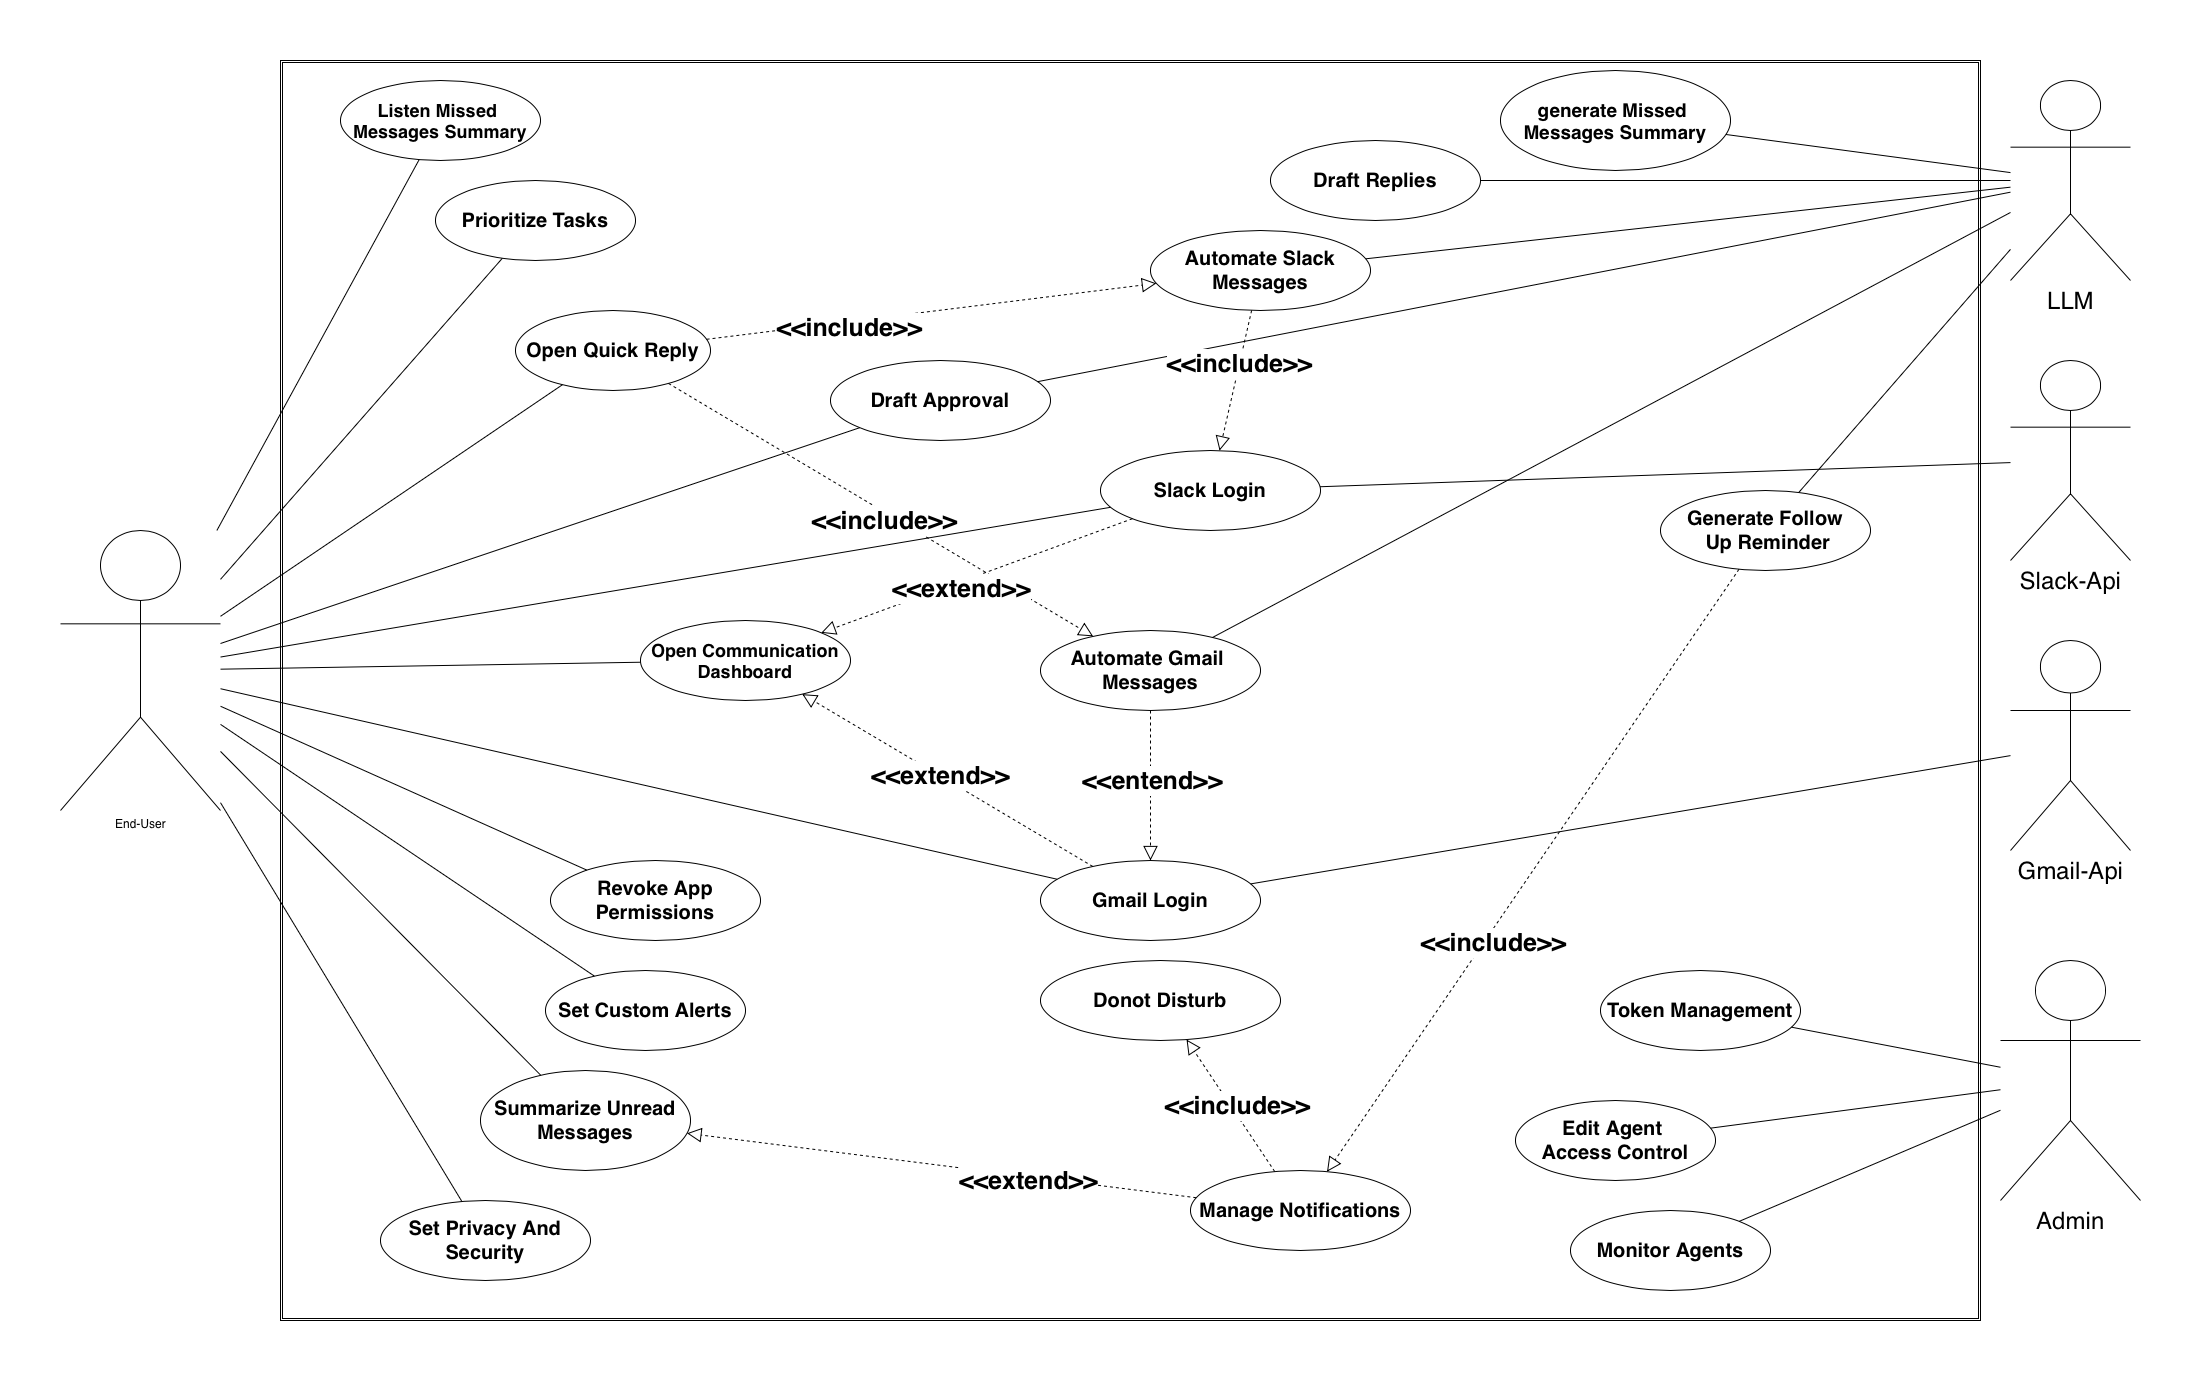
\includegraphics[width=\textwidth, height=0.83\textheight, keepaspectratio]{Figures/Usecase_Diagram.png}
  \caption[Use Case Diagram]{AutoReturn Use Case Diagram}
\end{figure}
\FloatBarrier

This diagram is intentionally centered on the practical behaviors that were implemented and tested in the final prototype. It avoids speculative functions and instead emphasizes the workflows that connect platform integration, assisted decision support, and user-controlled automation.

\section{Use Case Descriptions}
The following use cases describe the main user-facing workflows supported by the final AutoReturn prototype. Together, they show how the desktop interface, orchestration layer, and supporting services cooperate to produce controlled communication assistance.

\subsection{UC-01: Unified Inbox Management}
\textbf{Actor:} User \\
\textbf{Description:} The user views and manages consolidated messages from Gmail and Slack through a unified interface. \\
\textbf{Preconditions:} Gmail and Slack accounts are connected and authenticated. \\
\textbf{Main Flow:}
\begin{enumerate}
    \item The user opens the AutoReturn application.
    \item The system retrieves messages from connected platforms.
    \item The system displays the unified inbox with message summaries and priority indicators.
    \item The user filters, sorts, or searches messages.
    \item The user opens a message and decides whether to review, summarize, or respond.
\end{enumerate}
\textbf{Postconditions:} Messages remain available in the unified inbox and subsequent actions can be routed through the same workflow.

This use case represents the central entry point of the system because many other workflows begin from a message selected in the unified inbox. It therefore captures the practical value of AutoReturn as a workspace rather than as a set of disconnected features.

\subsection{UC-02: Draft and Reply Assistance}
\textbf{Actor:} User, System \\
\textbf{Description:} The system generates contextual response drafts and applies configured reply policies before any message is sent. \\
\textbf{Preconditions:} Draft generation or reply support is enabled for the connected platform. \\
\textbf{Main Flow:}
\begin{enumerate}
    \item The system receives or loads a message.
    \item The priority classification module determines the urgency level of the message.
    \item A model-backed service generates a contextual response draft.
    \item The tone preference module adjusts the response style.
    \item The system checks policy rules such as review-first mode, DND, and sender allowlists.
    \item The system either saves the draft for review or completes the reply path permitted by policy.
    \item The action is logged for user review.
\end{enumerate}
\textbf{Postconditions:} A response draft or controlled reply action is produced and recorded.

This use case is important because it combines several of the project’s core ideas in one flow: model-assisted drafting, tone adjustment, and policy-based control. It also shows how the system preserves user oversight when communication actions carry greater risk.

\subsection{UC-03: Voice-Assisted Control}
\textbf{Actor:} User \\
\textbf{Description:} The user interacts with the system using voice-assisted controls where supported by the current implementation. \\
\textbf{Preconditions:} A microphone is available and voice interaction features are enabled. \\
\textbf{Main Flow:}
\begin{enumerate}
    \item The user activates the voice interaction feature.
    \item The system accepts a spoken command.
    \item The command is converted into text for processing.
    \item The system interprets the requested action.
    \item The system executes the requested operation.
    \item The system provides feedback to the user.
\end{enumerate}
\textbf{Postconditions:} The requested command is processed and the user is informed of the result.

Although voice support is not the sole focus of the final prototype, it remains relevant as a supporting interaction pathway. This use case therefore reflects the intended role of voice as an extension of the desktop workflow rather than a separate conversational product.

\subsection{UC-04: Task Extraction and Management}
\textbf{Actor:} User, System \\
\textbf{Description:} The system analyzes incoming messages and extracts actionable information such as events, deadlines, or follow-up items for user review. \\
\textbf{Preconditions:} Extraction services are enabled for the current message workflow. \\
\textbf{Main Flow:}
\begin{enumerate}
    \item The system processes an incoming message.
    \item Model-assisted extraction analyzes the message for events, deadlines, or requested actions.
    \item The system structures the extracted information for review.
    \item The user reviews, edits, or confirms the extracted result.
    \item When relevant, the system prepares an exportable event or follow-up artifact.
\end{enumerate}
\textbf{Postconditions:} Actionable information is extracted and prepared for later use.

This workflow demonstrates how AutoReturn moves beyond message viewing and reply generation into actionable interpretation. It is particularly important for event handling, follow-up support, and other productivity-oriented extensions of communication analysis.

\subsection{UC-05: File Attachment Automation}
\textbf{Actor:} User, System \\
\textbf{Description:} The system identifies and attaches relevant files to outgoing responses based on user requests and file-matching logic. \\
\textbf{Preconditions:} File attachment automation is enabled and authorized directories are configured. \\
\textbf{Main Flow:}
\begin{enumerate}
    \item The system detects a file request in the outgoing message.
    \item The system searches configured directories for matching files.
    \item If a single match is found, the file is attached automatically.
    \item If multiple matches are found, the user is prompted to select the correct file.
    \item The selected file is attached to the outgoing response.
\end{enumerate}
\textbf{Postconditions:} The outgoing message is prepared with the correct file attachment.

This use case also illustrates the project’s emphasis on cautious automation. Rather than attaching files aggressively, the system is designed to stop and request confirmation when ambiguity would reduce trust or increase error risk.

\section{Activity Diagrams}
\noindent The activity diagrams summarize the highest-level workflows implemented in the current prototype. They illustrate control flow rather than every internal service call.
\Needspace{0.42\textheight}
\subsection{Overall System Activity}
\begin{figure}[H]
  \centering
  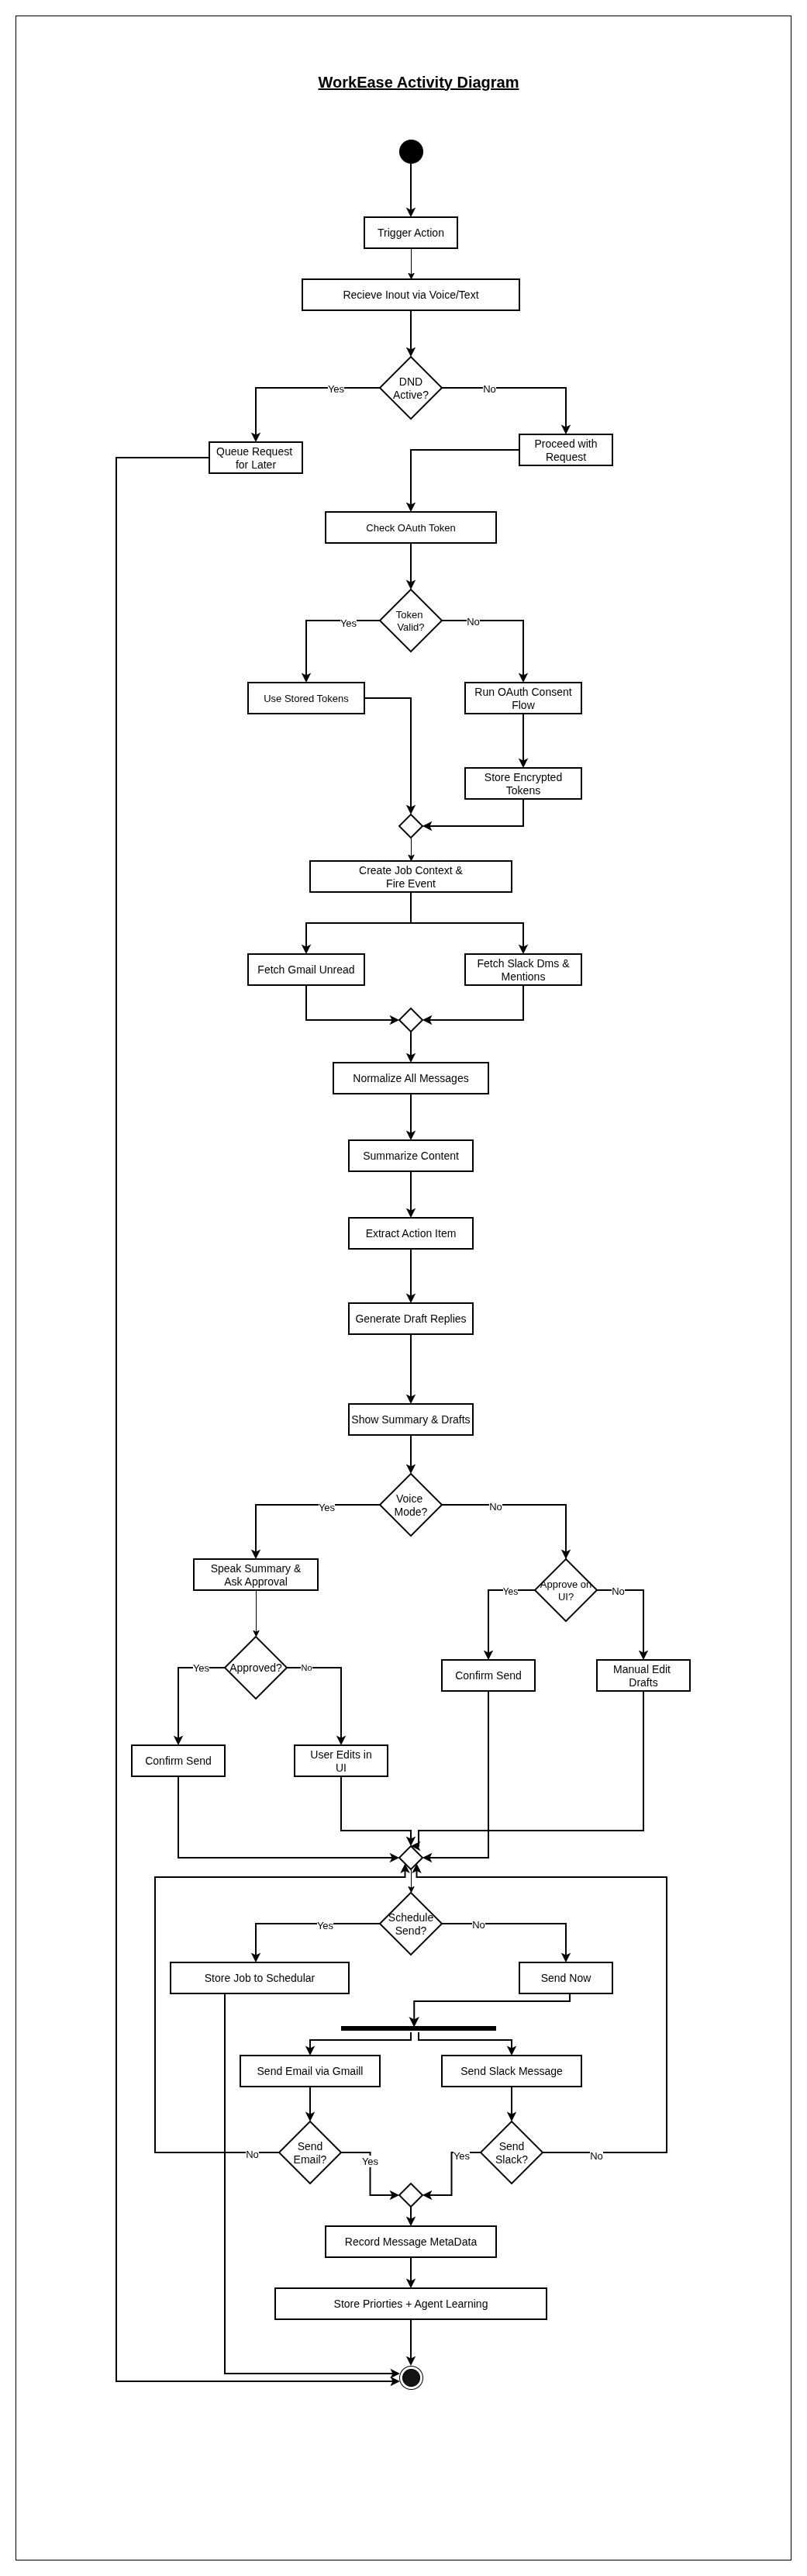
\includegraphics[width=\textwidth, height=0.76\textheight, keepaspectratio]{Figures/Complete_Activity_Diagram.png}
  \caption[System Activity Diagram]{Overall System Activity Diagram}
\end{figure}
\FloatBarrier

The overall activity diagram is useful because it compresses the major workflow stages into one view, from message intake to assisted action. It helps explain how the system coordinates retrieval, analysis, policy checks, and output preparation as one connected flow.

\Needspace{0.38\textheight}
\subsection{Activity 1: Voice-Based Interaction and Control}
\begin{figure}[H]
  \centering
  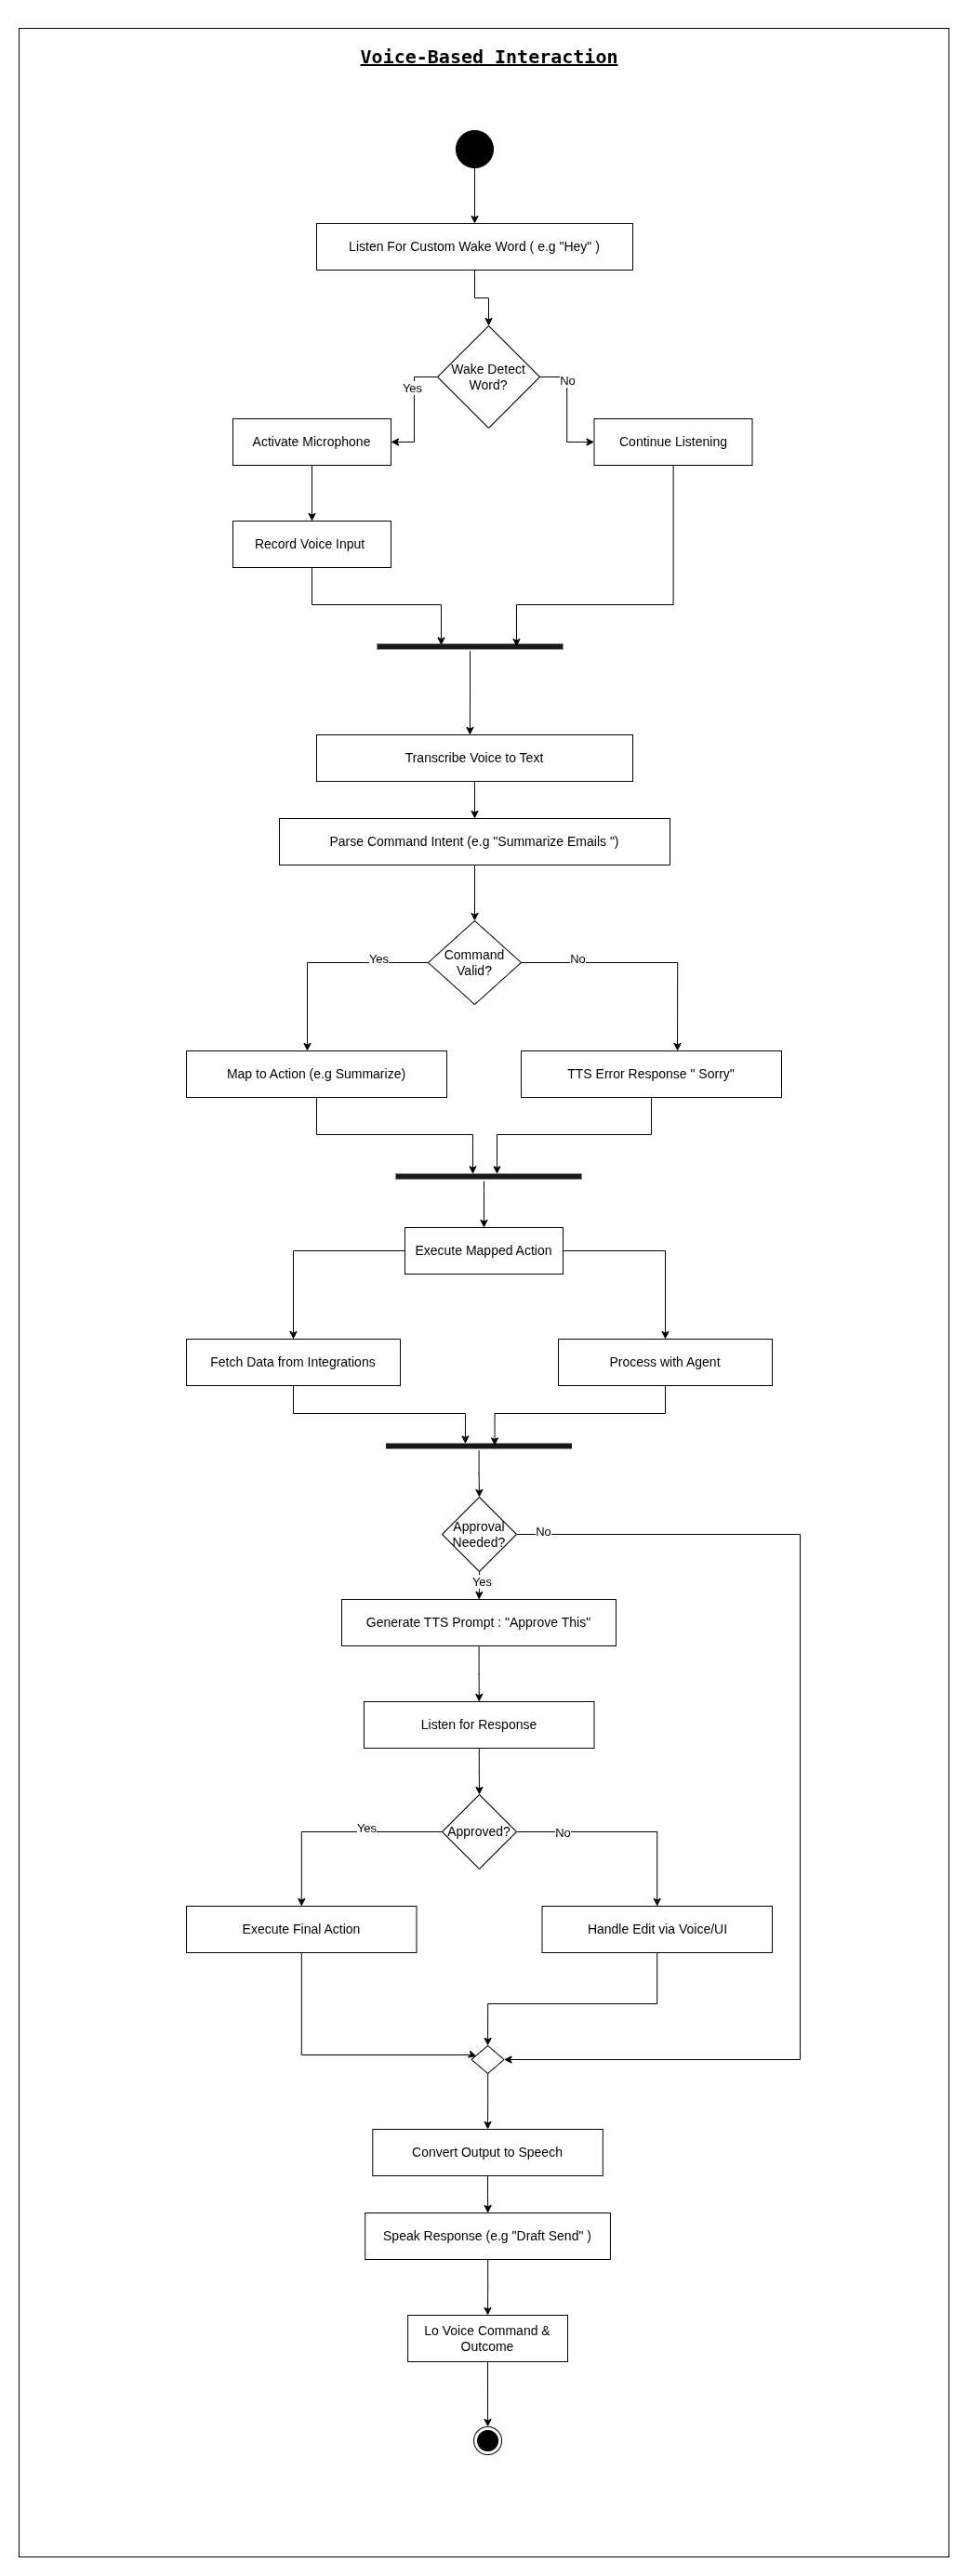
\includegraphics[width=\textwidth, height=0.72\textheight, keepaspectratio]{Figures/Activity_1_Voice_Based_Interaction.png}
  \caption[Voice Interaction Activity Diagram]{Voice Interaction Activity Diagram}
\end{figure}
\FloatBarrier

This activity emphasizes the narrower but still meaningful role of voice support in the final system. It shows that voice is treated as a controlled trigger for supported actions rather than as the sole interaction model.

\Needspace{0.38\textheight}
\subsection{Activity 2: Smart Email and Message Automation}
\begin{figure}[H]
  \centering
  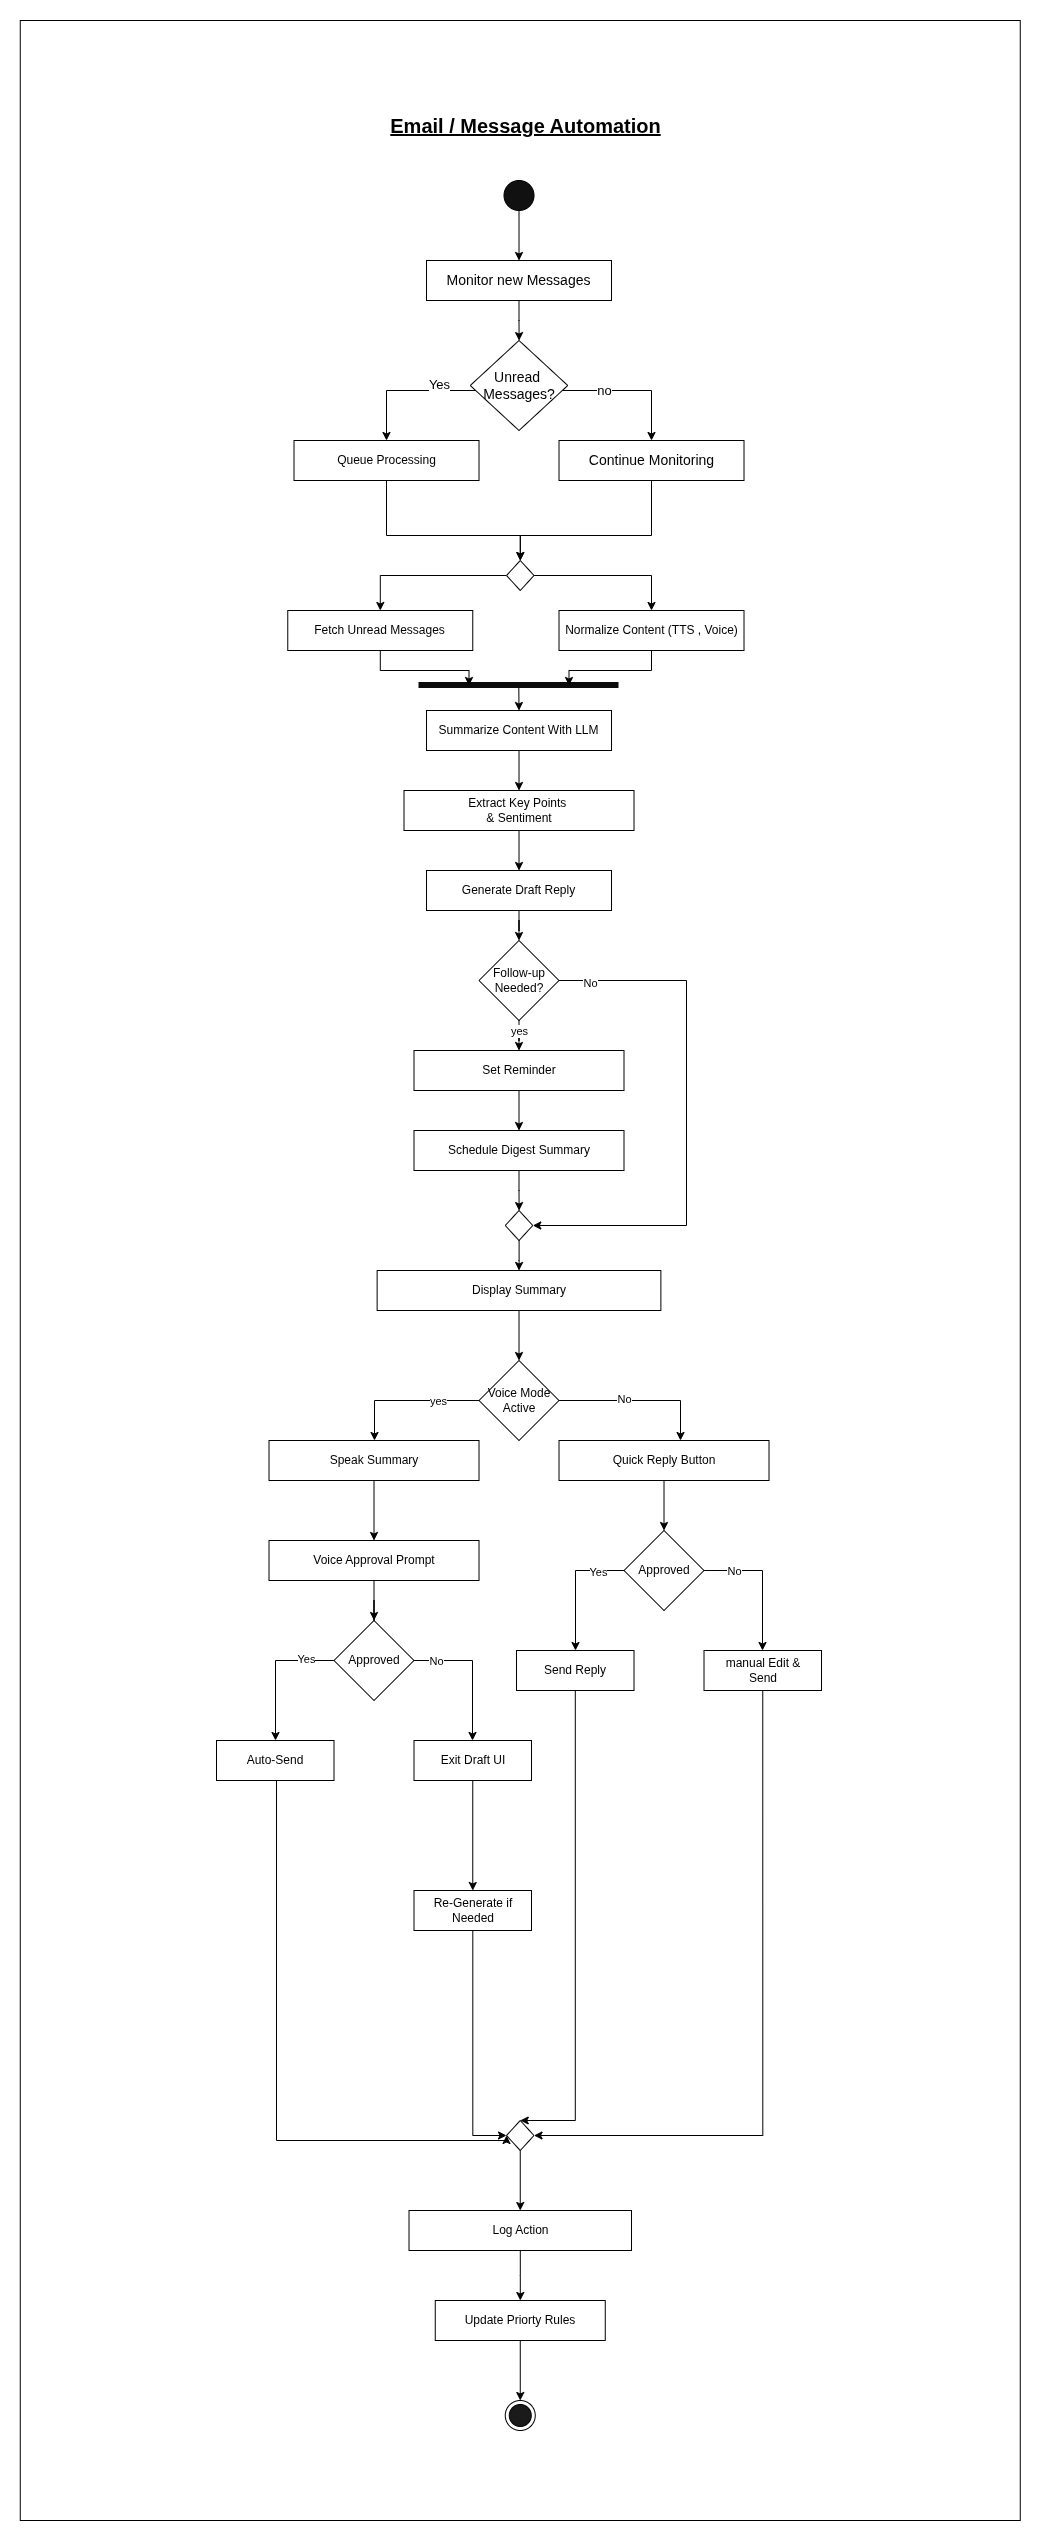
\includegraphics[width=\textwidth, height=0.72\textheight, keepaspectratio]{Figures/Activity_2_Email_Message_Automation.png}
  \caption[Smart Automation Activity Diagram]{Smart Email and Message Automation Activity Diagram}
\end{figure}
\FloatBarrier

This diagram is important because it captures the project’s most representative intelligent workflow: receiving a message, analyzing it, generating support artifacts, and applying user-governed response rules. It therefore reflects the practical center of the implementation.

\Needspace{0.36\textheight}
\subsection{Activity 3: Multi-App Integration and Authentication}
\begin{figure}[H]
  \centering
  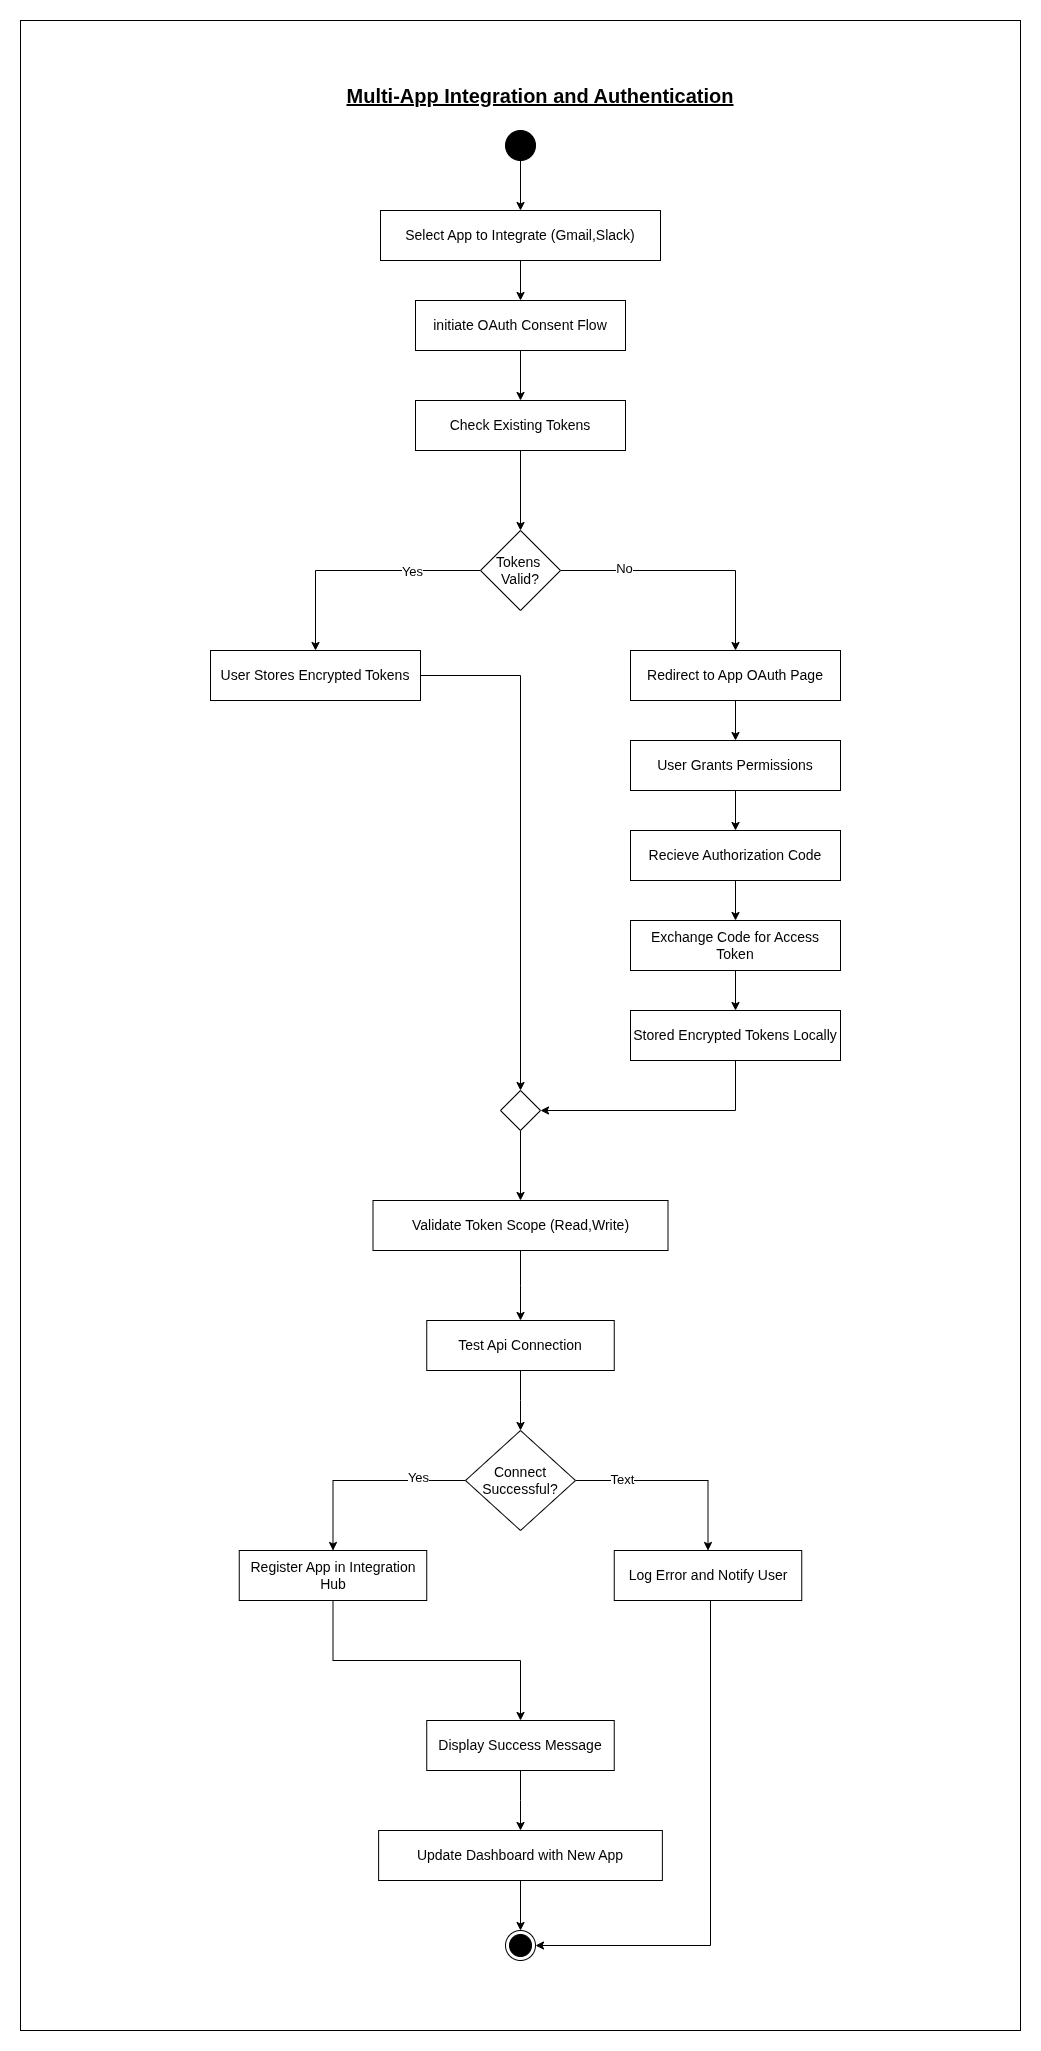
\includegraphics[width=\textwidth, height=0.70\textheight, keepaspectratio]{Figures/Activity_3_MultiApp_Integration.png}
  \caption[Multi-App Activity Diagram]{Multi-App Integration Activity Diagram}
\end{figure}
\FloatBarrier

The multi-app activity also highlights why the orchestrator-agent design was necessary. Different platforms must be normalized and coordinated before later intelligent services can operate consistently across them.

Together, these diagrams show that the system is organized around repeatable workflow stages rather than isolated feature calls. This process view is important for understanding how AutoReturn coordinates retrieval, analysis, user review, and controlled action.

\section{Component Diagram}
\noindent Figure 4.6 presents the major implementation blocks and their interaction boundaries.
\begin{figure}[htbp]
  \centering
  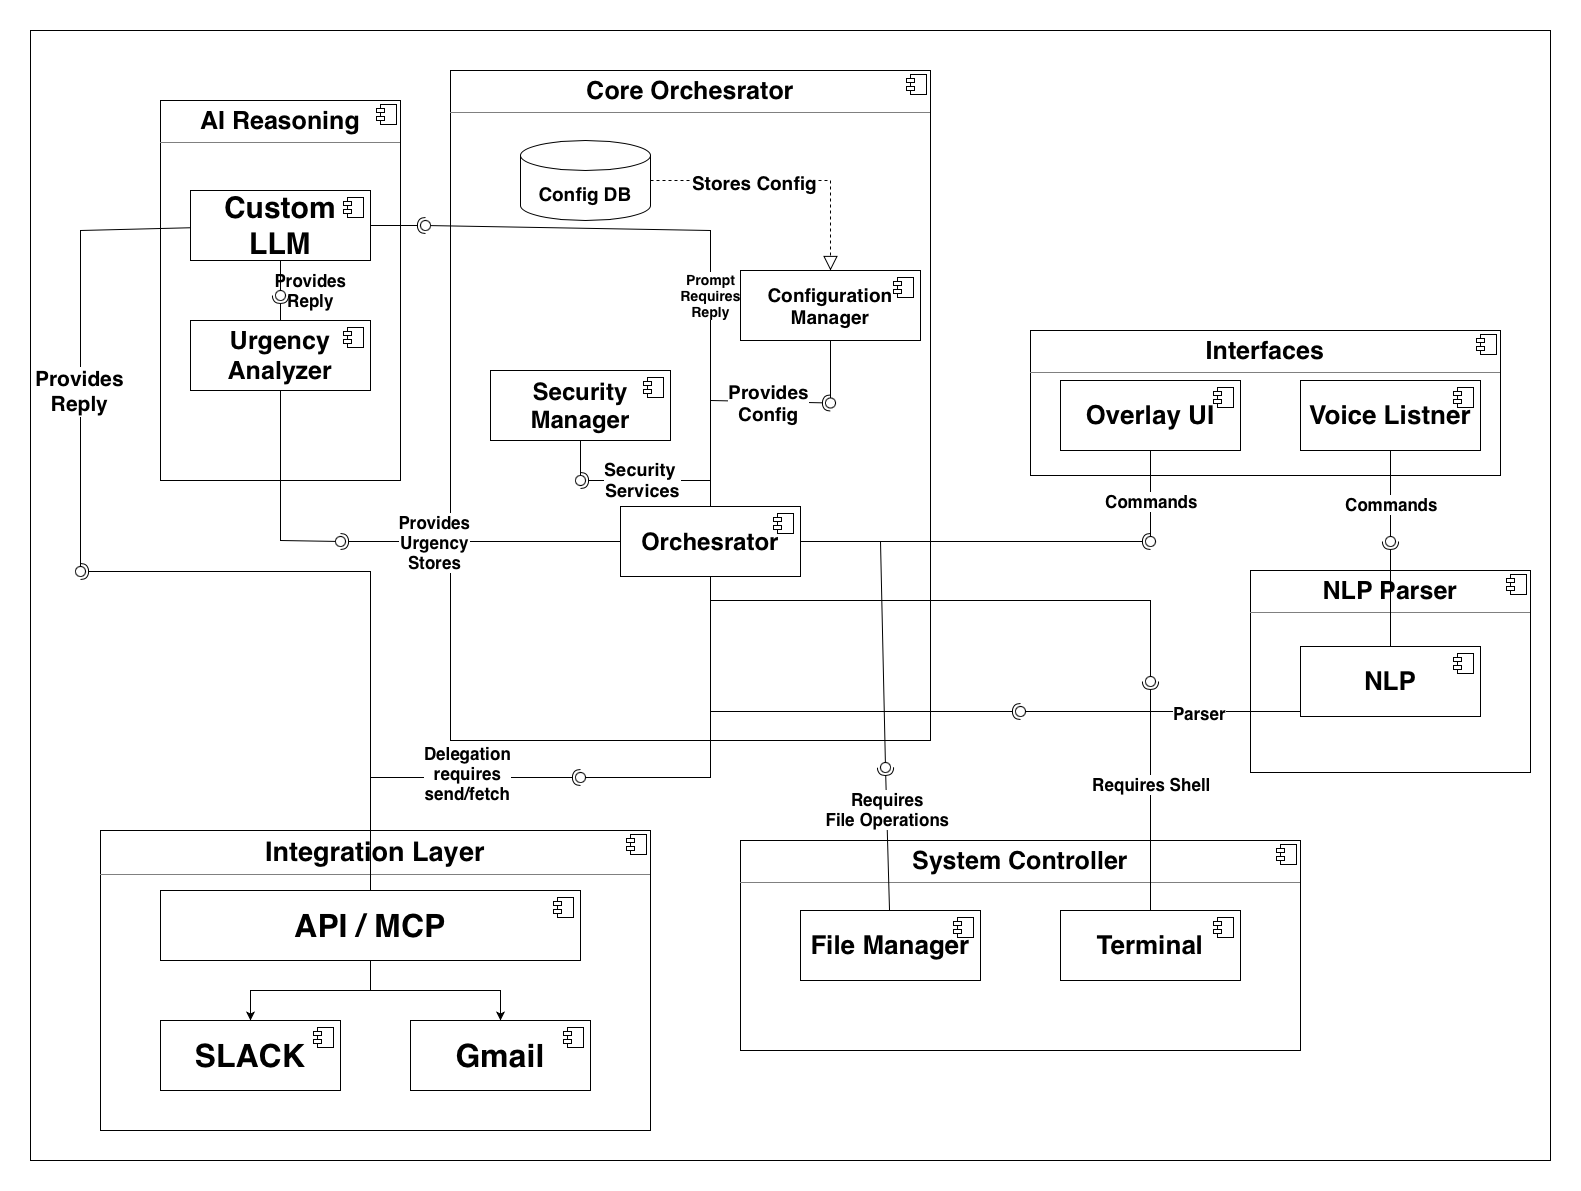
\includegraphics[width=\textwidth, height=0.90\textheight, keepaspectratio]{Figures/Component.png}
  \caption[Component Diagram]{AutoReturn Component Diagram}
\end{figure}
\FloatBarrier

The component view complements the earlier behavioral diagrams by showing how those workflows are distributed across the main software units. It also highlights the separation between interface concerns, orchestration logic, platform agents, and supporting backend services.

\section{Architecture Diagram}
\noindent The architecture diagram emphasizes the final desktop-oriented structure: a PySide6 user interface, an orchestration layer, platform agents, and shared processing services.
\begin{figure}[!htbp]
    \centering
    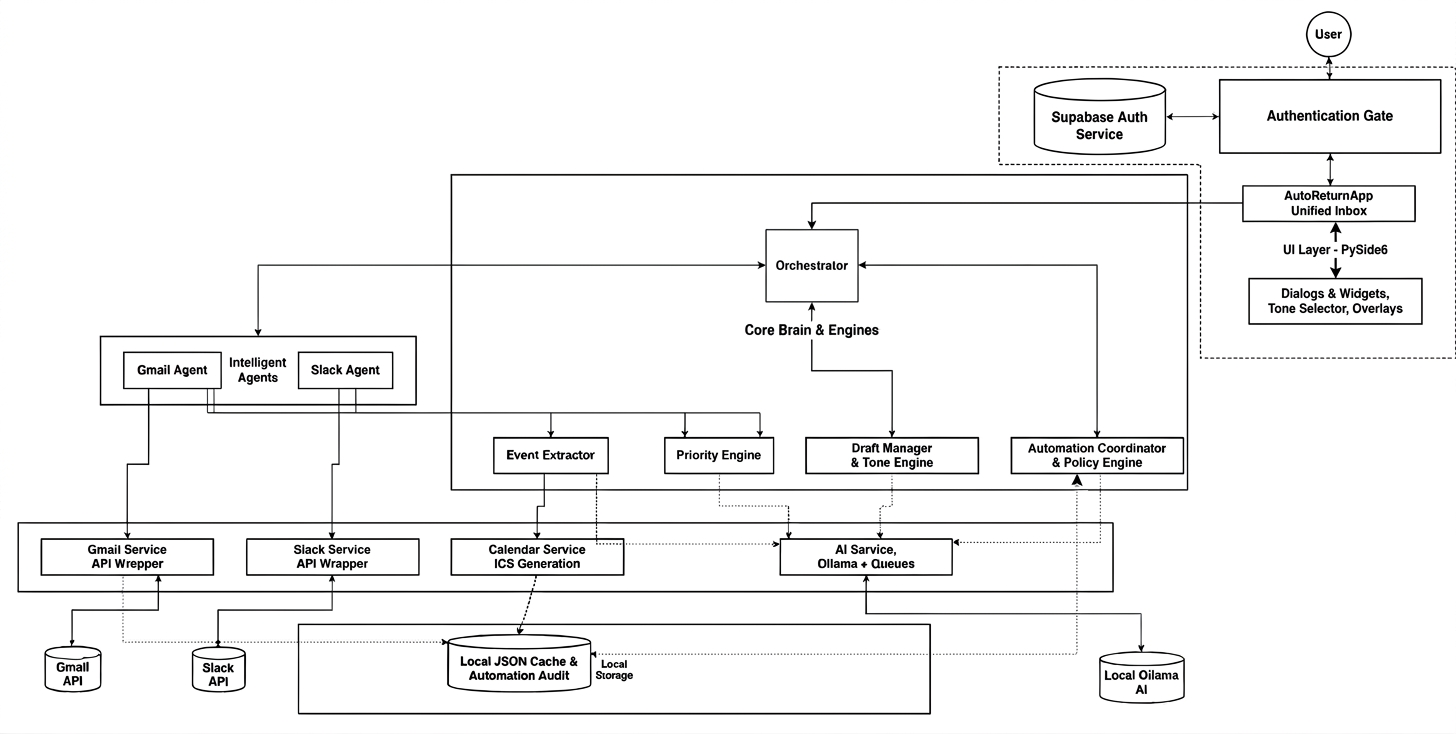
\includegraphics[width=1.08\textwidth]{Figures/Architecture5.png}
    \caption[System Architecture]{AutoReturn System Architecture}
    \label{fig:architecture}
\end{figure}

This architectural perspective is especially useful because AutoReturn depends on coordination between several subsystems rather than on a single processing pipeline. The diagram therefore reinforces the modular design rationale introduced in the earlier chapters.

\section{Wireframes}
\noindent The wireframes in this section present the intended interaction layout of the AutoReturn desktop interface. They complement the structural diagrams by showing how unified inbox navigation, assisted reply handling, notifications, and voice entry points were organized at the interface level.

\subsection{Unified Workspace Wireframe}
\begin{figure}[!htbp]
    \centering
    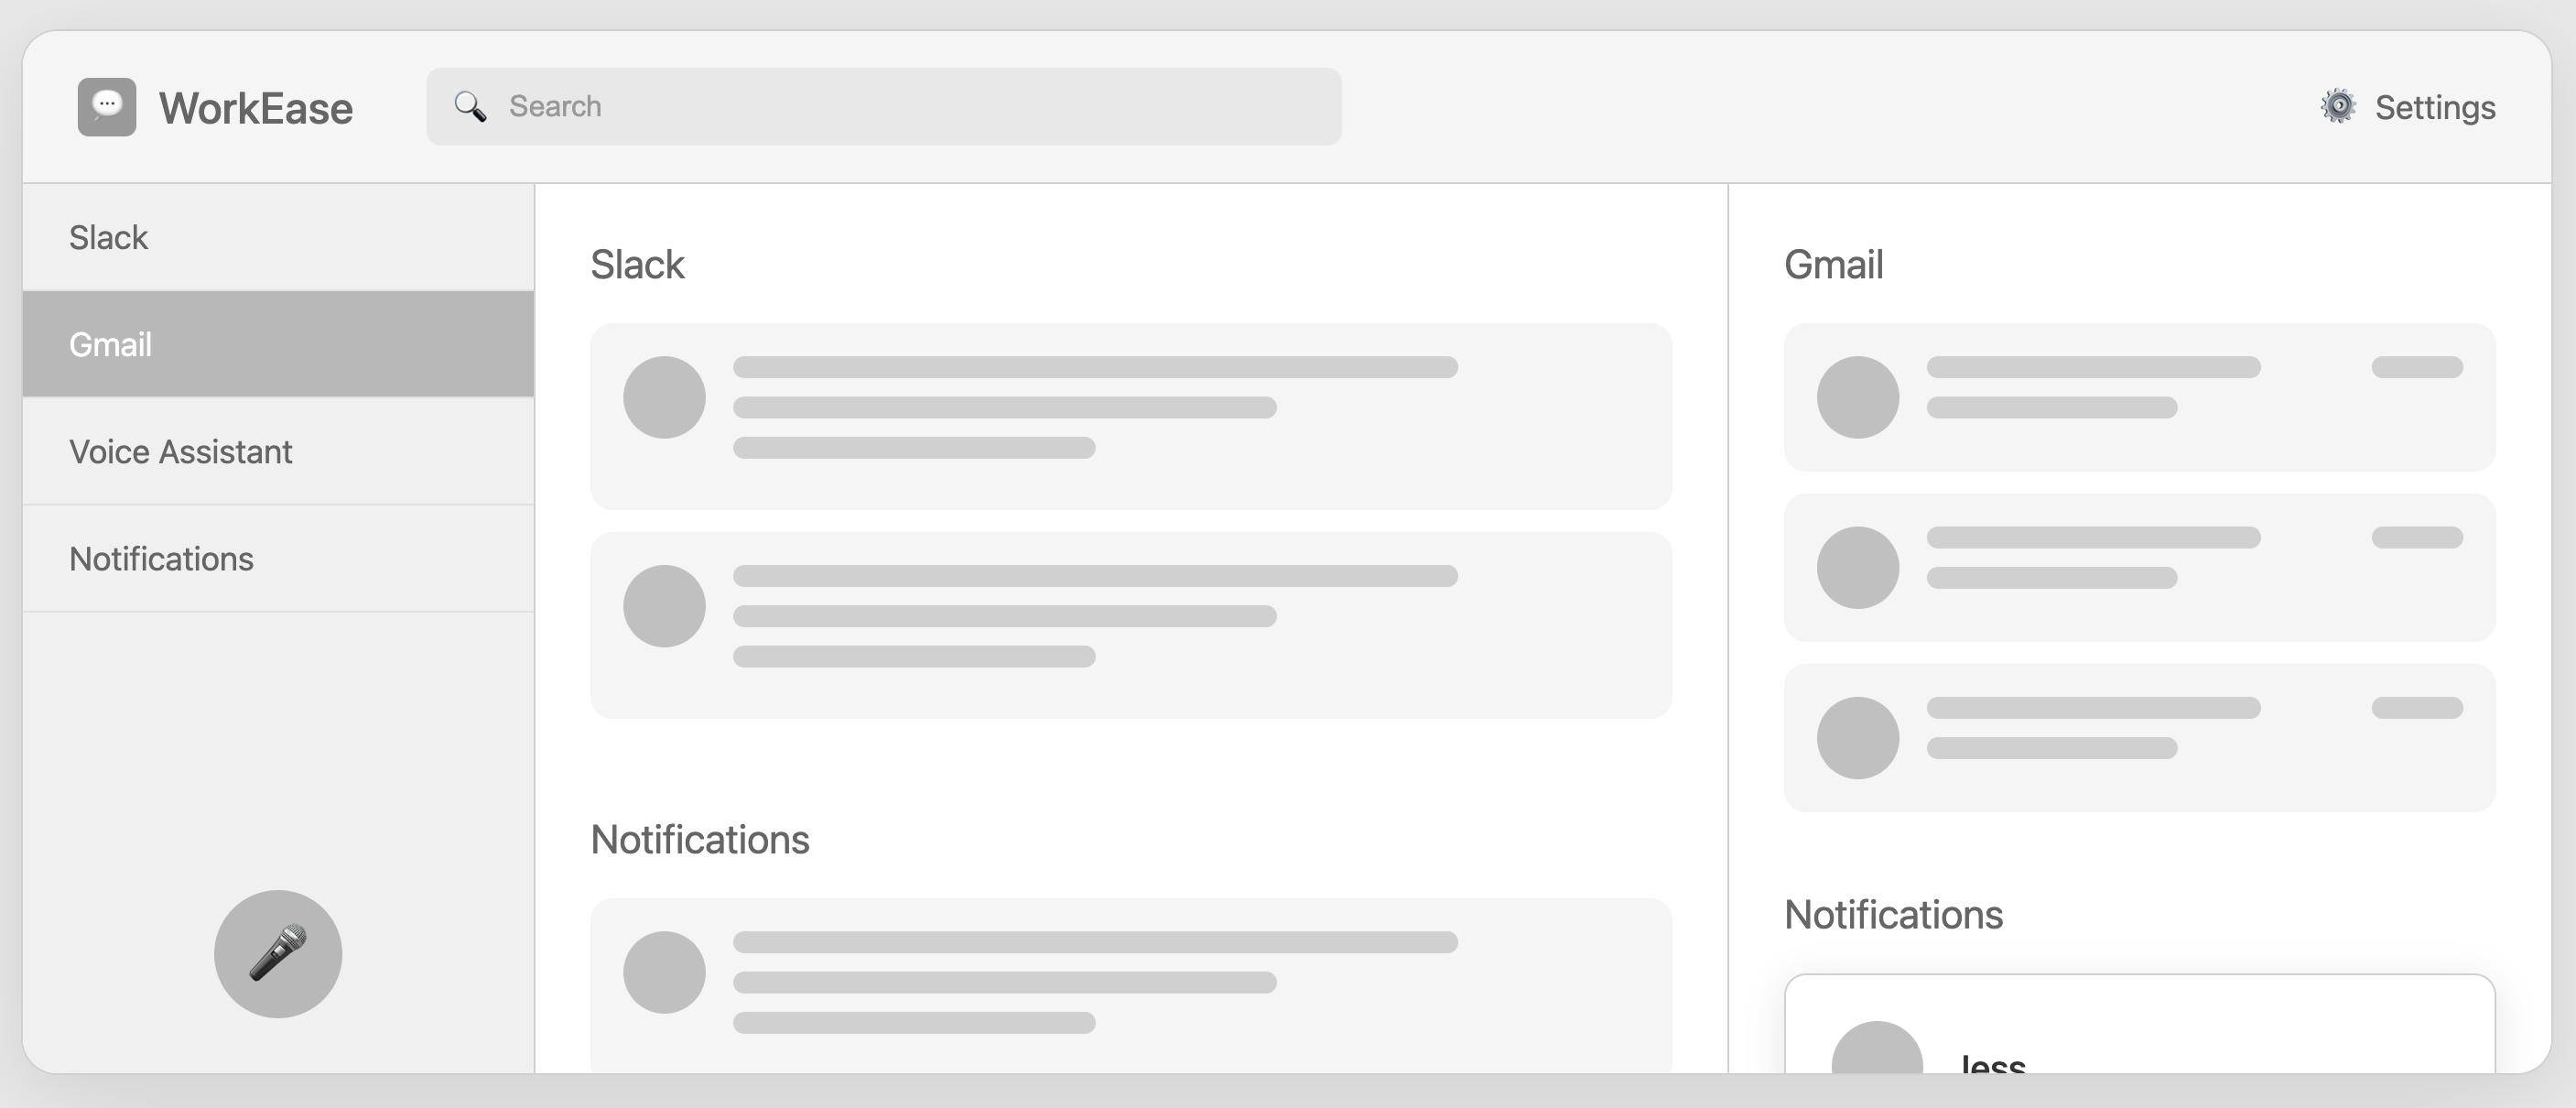
\includegraphics[width=1.03\textwidth]{Figures/Wireframe2.png}
\caption[Unified Workspace Wireframe]{AutoReturn Unified Workspace Wireframe}
\label{fig:wireframe_workspace}
\end{figure}

This wireframe helps show how the technical goals of unification, visibility, and assisted action are translated into one main working screen. It therefore provides an interface-level interpretation of the architectural and workflow diagrams presented earlier.

\subsection{Notification and Assisted Reply Wireframe}
\begin{figure}[!htbp]
    \centering
    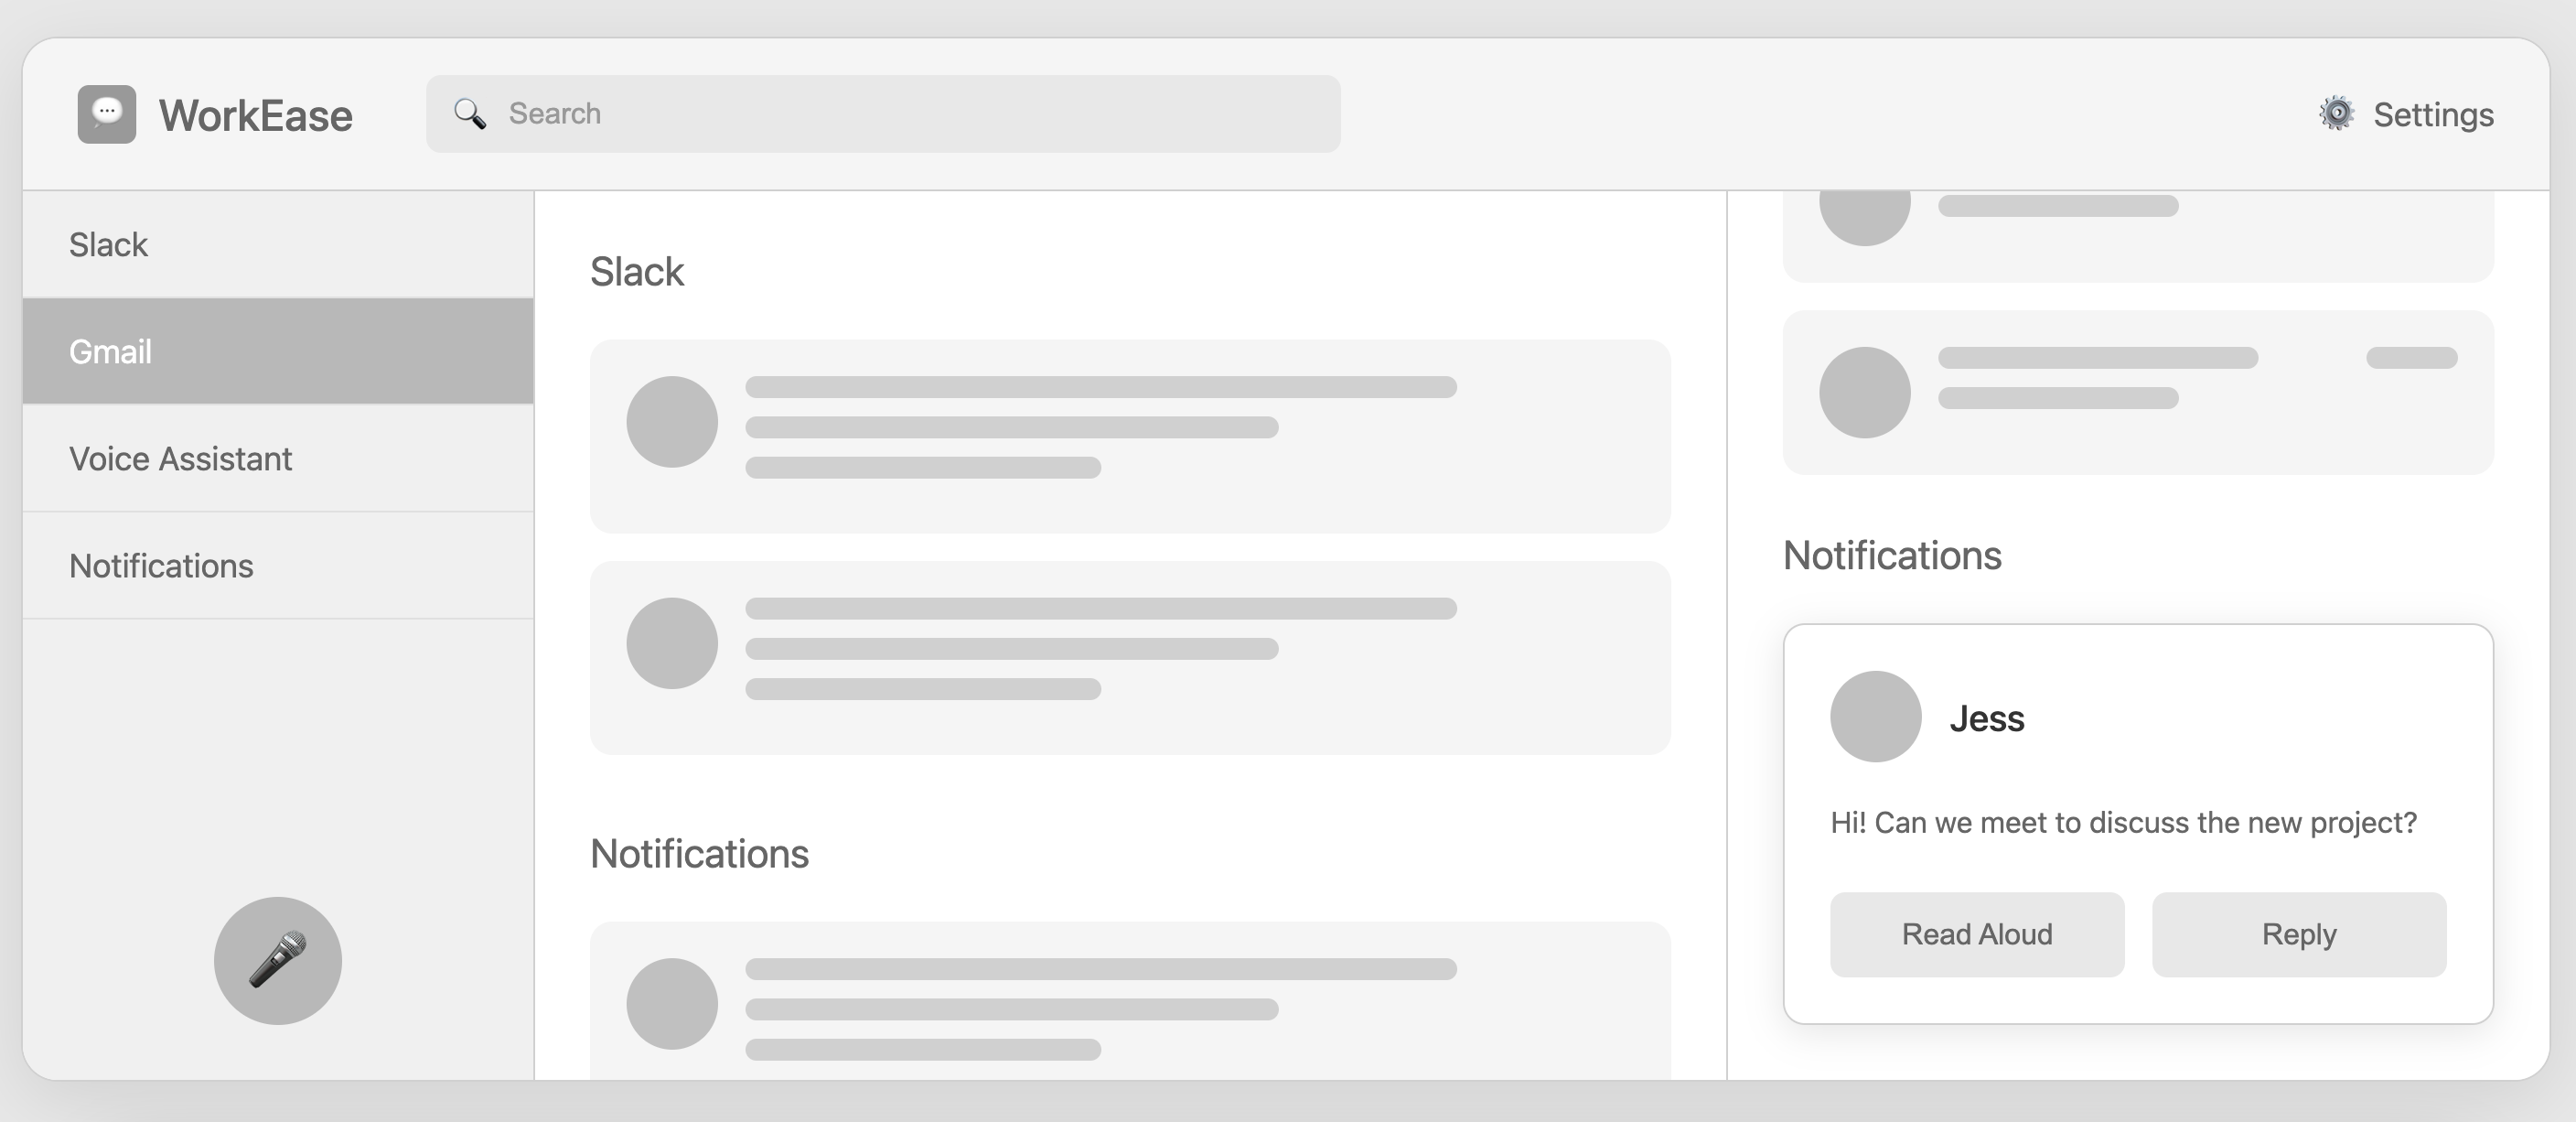
\includegraphics[width=1.03\textwidth]{Figures/wireframe1.png}
    \caption[Reply Assistant Wireframe]{Notification and Reply Wireframe}
    \label{fig:wireframe_reply}
\end{figure}

These wireframes are included to show how the technical architecture becomes visible to the user as a coherent workspace. They therefore bridge the gap between the abstract system model and the practical layout of the implemented interface.

\section{Modeling Discussion}
The modeling view presented in this chapter reflects the final prototype more accurately than the earlier concept-stage architecture. AutoReturn is best understood as a desktop system with a unified interface, an orchestration layer, platform agents, policy services, and model-assisted support components. The structural diagrams explain the underlying workflow, while the wireframes show how these functions are surfaced to the user in the desktop application.

Viewed together, the modeling artifacts provide a balanced description of the system from functional, behavioral, structural, and interface perspectives. This is more useful for the current project than a narrowly code-centric model because AutoReturn’s value lies in coordinated workflow behavior across multiple services.

\chapter{Implementation}
\label{sec:implementation}

\section{Implementation Overview}
AutoReturn was implemented as a native \textbf{PySide6} desktop application with a modular backend centered on an \textbf{Orchestrator} class \cite{pyside2024}. The implementation combines platform-specific agents, configurable automation services, and model-assisted processing for summarization, drafting, extraction, and tone-aware assistance. Gmail and Slack connectivity rely on the official platform APIs \cite{gmail2023,slack2023}, while account ownership and authentication are coordinated through a Supabase-backed identity layer \cite{supabase2024}. The final codebase prioritizes controllable automation over fully autonomous behavior, so high-risk actions are still guarded by explicit policy checks, confidence rules, or user review steps.

This chapter focuses on the final implemented state of the system rather than on intermediate concepts from earlier project phases. It therefore summarizes the completed modules, the main engineering challenges, the recurring implementation patterns, and the interface views that best represent the final prototype.

\section{Module Details}
This section summarizes the final implemented modules so that the report can connect design claims with concrete development outcomes. The following tables provide a compact view of the completed functionality present in the final AutoReturn prototype.

\begin{table}[!htbp]
\centering
\caption{AutoReturn Module Details -- Part I}
\label{tab:implementation}
\footnotesize
\renewcommand{\arraystretch}{1.15}
\setlength{\tabcolsep}{5pt}
\begin{adjustbox}{width=\textwidth}
\begin{tabular}{|>{\raggedright\arraybackslash}p{4.8cm}|>{\raggedright\arraybackslash}p{8.7cm}|}
\hline
\textbf{Module} & \textbf{Implementation Details} \\
\hline
Priority of email/message & Weighted urgency assessment combines keyword, deadline, and sender signals through the priority engine. \\
\hline
Email/message summary & AI-assisted summaries are generated for synchronized Gmail and Slack messages through the model-backed service layer. \\
\hline
Draft generation & Draft generation is integrated into the unified workflow and supports downstream review, tone adjustment, and policy checks. \\
\hline
Plain text response & Plain-reply review dialogs and policy-aware sending are implemented for controlled response workflows. \\
\hline
Task classification & Model-assisted task and intent classification is integrated into the automation workflow for actionable message understanding. \\
\hline
Task extraction & Structured task and event extraction are supported for messages that contain actionable or schedulable content. \\
\hline
Unified inbox & Gmail and Slack content is normalized into a shared message flow for display and downstream processing. \\
\hline
Orchestrator & A central orchestrator coordinates routing, shared services, and platform-specific agent interaction. \\
\hline
Gmail agent & Message retrieval, reading, summarization, drafting, and automation support are integrated through the Gmail agent. \\
\hline
Slack agent & Slack message retrieval, unified-inbox integration, and downstream workflow support are implemented through the Slack agent. \\
\hline
Tone preference & Tone recommendation and draft adjustment are handled through the tone engine with configurable preferences and conservative fallbacks. \\
\hline
Event-driven file lookup & The attachment resolver searches approved paths, blocks ambiguous auto-attachment, and requests manual confirmation when needed. \\
\hline
Search & Search is supported across the desktop workflow and is also integrated into voice-triggered UI actions. \\
\hline
\end{tabular}
\end{adjustbox}
\end{table}

\begin{table}[!htbp]
\centering
\caption{AutoReturn Module Details -- Part II}
\footnotesize
\renewcommand{\arraystretch}{1.15}
\setlength{\tabcolsep}{5pt}
\begin{adjustbox}{width=\textwidth}
\begin{tabular}{|>{\raggedright\arraybackslash}p{4.8cm}|>{\raggedright\arraybackslash}p{8.7cm}|}
\hline
\textbf{Module} & \textbf{Implementation Details} \\
\hline
Desktop and pop-up notifications & Notification dialogs, unread tracking, and controlled desktop-alert behavior are implemented in the desktop client. \\
\hline
Website and deployment & A public project website is available and deployed for presentation and external project overview purposes. \\
\hline
.deb package & Packaging support is included as part of the deliverable direction for installation and distribution of the desktop application. \\
\hline
Sender statistics & Sender and tone-related usage statistics are available through the settings and tone-profile interfaces. \\
\hline
Calendar feature & Event extraction, conflict checks, Google Calendar insertion, and ICS export are implemented for scheduling workflows. \\
\hline
CI/CD pipeline & Structured validation and project-delivery workflow support are included as part of the final implementation and deployment process. \\
\hline
Auto reply & Auto-reply mode is implemented through the automation policy engine and remains gated by DND and policy checks. \\
\hline
DND & Do Not Disturb rules suppress or redirect response and notification behavior according to user policy settings. \\
\hline
Voice-enabled actions & Voice support includes transcription, hotkey activation, wake-mode support, and controlled UI actions within the desktop workflow. \\
\hline
Wake-word activation & Wake-word mode is supported through the integrated ``Hey AutoReturn'' activation phrase for hands-free triggering. \\
\hline
\end{tabular}
\end{adjustbox}
\end{table}

\section{Selected Technical Challenges and Solutions}
The implementation process required repeated refinement in response to ambiguity, cross-platform mismatch, and automation safety concerns. Table~\ref{tab:technical_challenges} summarizes the most important engineering challenges encountered during development and the responses adopted in the final system.

\begin{table}[!htbp]
\centering
\footnotesize
\renewcommand{\arraystretch}{1.15}
\setlength{\tabcolsep}{5pt}
\begin{adjustbox}{width=\textwidth}
\begin{tabular}{|>{\raggedright\arraybackslash}p{0.8cm}|>{\raggedright\arraybackslash}p{3.2cm}|>{\raggedright\arraybackslash}p{5.1cm}|>{\raggedright\arraybackslash}p{6.1cm}|}
\hline
\textbf{No.} & \textbf{Challenge} & \textbf{Issue} & \textbf{Implemented Response} \\ \hline
1 & Platform authentication & Gmail and Slack integration required reliable token handling and account state management. & OAuth refresh logic, account linking, and controlled authentication services were added so connected platforms could be reused safely across sessions. \\ \hline
2 & Priority ambiguity & Simple keyword matches produced weak urgency judgments, especially in negated phrases such as ``not urgent.'' & A weighted priority engine was introduced to combine keyword, deadline, and sender signals rather than relying on isolated words. \\ \hline
3 & Long-message context loss & Important requests were sometimes diluted inside long threads or mixed conversation history. & Message-cleaning and context-selection steps were added before summarization, drafting, and extraction workflows. \\ \hline
4 & Cross-platform data mismatch & Gmail and Slack expose different message structures, metadata, and identifiers. & The orchestrator normalizes content into a shared message flow so downstream services can operate consistently across both integrations. \\ \hline
5 & UI and worker concurrency & Background workers, API requests, and interface updates could interfere with one another. & Threaded execution and signal-based update paths were used to isolate slower tasks from the main interface. \\ \hline
6 & Tone-detection variability & Real-world language did not fit a purely rule-based formal/informal split. & The tone engine uses configurable rules and weighted signals, with conservative fallbacks when certainty is low. \\ \hline
7 & Attachment ambiguity & File requests could produce either no match or several plausible matches. & The attachment resolver blocks automatic completion when confidence is weak and requests manual confirmation instead. \\ \hline
8 & Reply policy safety & Automation should not treat every sender or message type equally. & Reply-policy services enforce DND, allowlists, and review-first modes before message transmission is allowed. \\ \hline
\end{tabular}
\end{adjustbox}
\caption{Selected Technical Challenges and Solutions}
\label{tab:technical_challenges}
\end{table}

\section{Implementation Patterns}
The implementation patterns in this section describe the recurring ways in which AutoReturn coordinates agents, routing logic, and assisted interaction. These patterns are important because they explain how the completed features operate together as one workflow-oriented desktop system.

\subsection{Orchestrator-Agent Coordination}
The backend is organized around an \textbf{Orchestrator} that routes work to platform-specific agents and shared services. In the current implementation, Gmail and Slack are the two primary agents, while drafting, tone recommendation, and automation settings are managed through dedicated backend components. This structure kept platform-specific logic separate from shared workflow logic and made it easier to evolve the system without rewriting the full request pipeline.

Event-related workflows also follow a standardized export path: when the system confirms a time-related item, it can prepare an ICS artifact aligned with the iCalendar interchange format \cite{rfc5545}.

\subsection{Priority Scoring}
The priority engine uses a weighted score rather than a single hard-coded rule. In simplified form, the implemented pattern can be described as:
\[
\text{urgency} = (w_k \times \text{keyword}) + (w_d \times \text{deadline}) + (w_s \times \text{sender})
\]
This design made the classifier more robust than simple keyword spotting because sender context and deadline cues can raise or lower the final urgency level.

The importance of this pattern lies in its balance between simplicity and usefulness. It provides an interpretable scoring approach that is easier to reason about than a fully opaque classifier, while still being richer than isolated keyword matching.

\subsection{Voice Command Handling}
Voice functionality is implemented as a supporting subsystem rather than the primary interaction model. The current codebase provides push-to-talk capture, transcription, wake-command parsing, and routing of recognized commands into controlled UI actions or orchestrator requests. Speech recognition in the project follows the practical desktop pattern enabled by Whisper-based tooling for local transcription workflows \cite{whisper2023}. This is useful for assisted interaction, but it is intentionally narrower than a fully conversational voice assistant.

This limited but structured role is consistent with the overall project philosophy of controlled assistance. Voice is included where it can support productivity, but it is not allowed to undermine reliability or clarity in the main communication workflows.

\section{Representative Code Snippets}
The following excerpts are intentionally brief and are included only to illustrate recurring implementation ideas from the final repository. They do not attempt to reproduce large portions of the source code, but instead show how key architectural patterns are expressed in practice.

\subsection{Base Agent Interface}
The actual backend agents share a small common contract. The report includes a shortened version of the implemented base class to illustrate this pattern:
\begin{verbatim}
class BaseAgent(ABC):
    def __init__(self, name: str):
        self.name = name

    @abstractmethod
    async def process_request(self, request):
        pass
\end{verbatim}

\subsection{Priority Engine Pattern}
The implemented priority engine follows the weighted three-signal structure shown below:
\begin{verbatim}
urgency = (w_keyword * k_score) + \
          (w_deadline * d_score) + \
          (w_sender * s_score)
\end{verbatim}
This compact pattern is more faithful to the final repository than the longer earlier pseudocode and better reflects how urgency labels are derived in practice.

Including this compact excerpt is useful because it shows that the implementation logic is not only described narratively in the report, but also reflected directly in the code structure. It therefore links the design explanation with the actual computational pattern used in the prototype.

\section{User Interface Screens}
The following figures present the principal user-interface screens of the AutoReturn desktop application. Together, they illustrate account connection, unified inbox navigation, assisted reply handling, automation settings, event workflows, and voice-related interaction points in the implemented system.

\begin{figure}[htbp]
    \centering
    \begin{subfigure}[t]{0.48\textwidth}
        \centering
        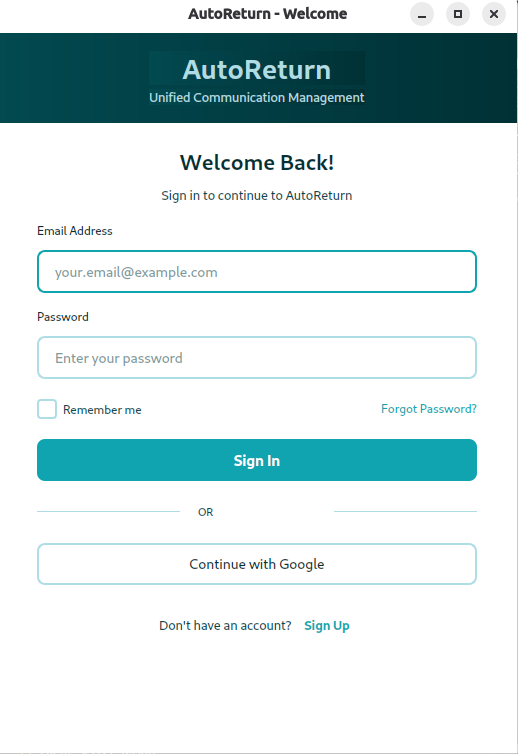
\includegraphics[width=0.70\linewidth,height=5.0cm,keepaspectratio]{Figures/Login_and_Account_Connection.png}
        \caption{Login and Account Connection}
        \label{fig:ui_login_connection}
    \end{subfigure}
    \hfill
    \begin{subfigure}[t]{0.48\textwidth}
        \centering
        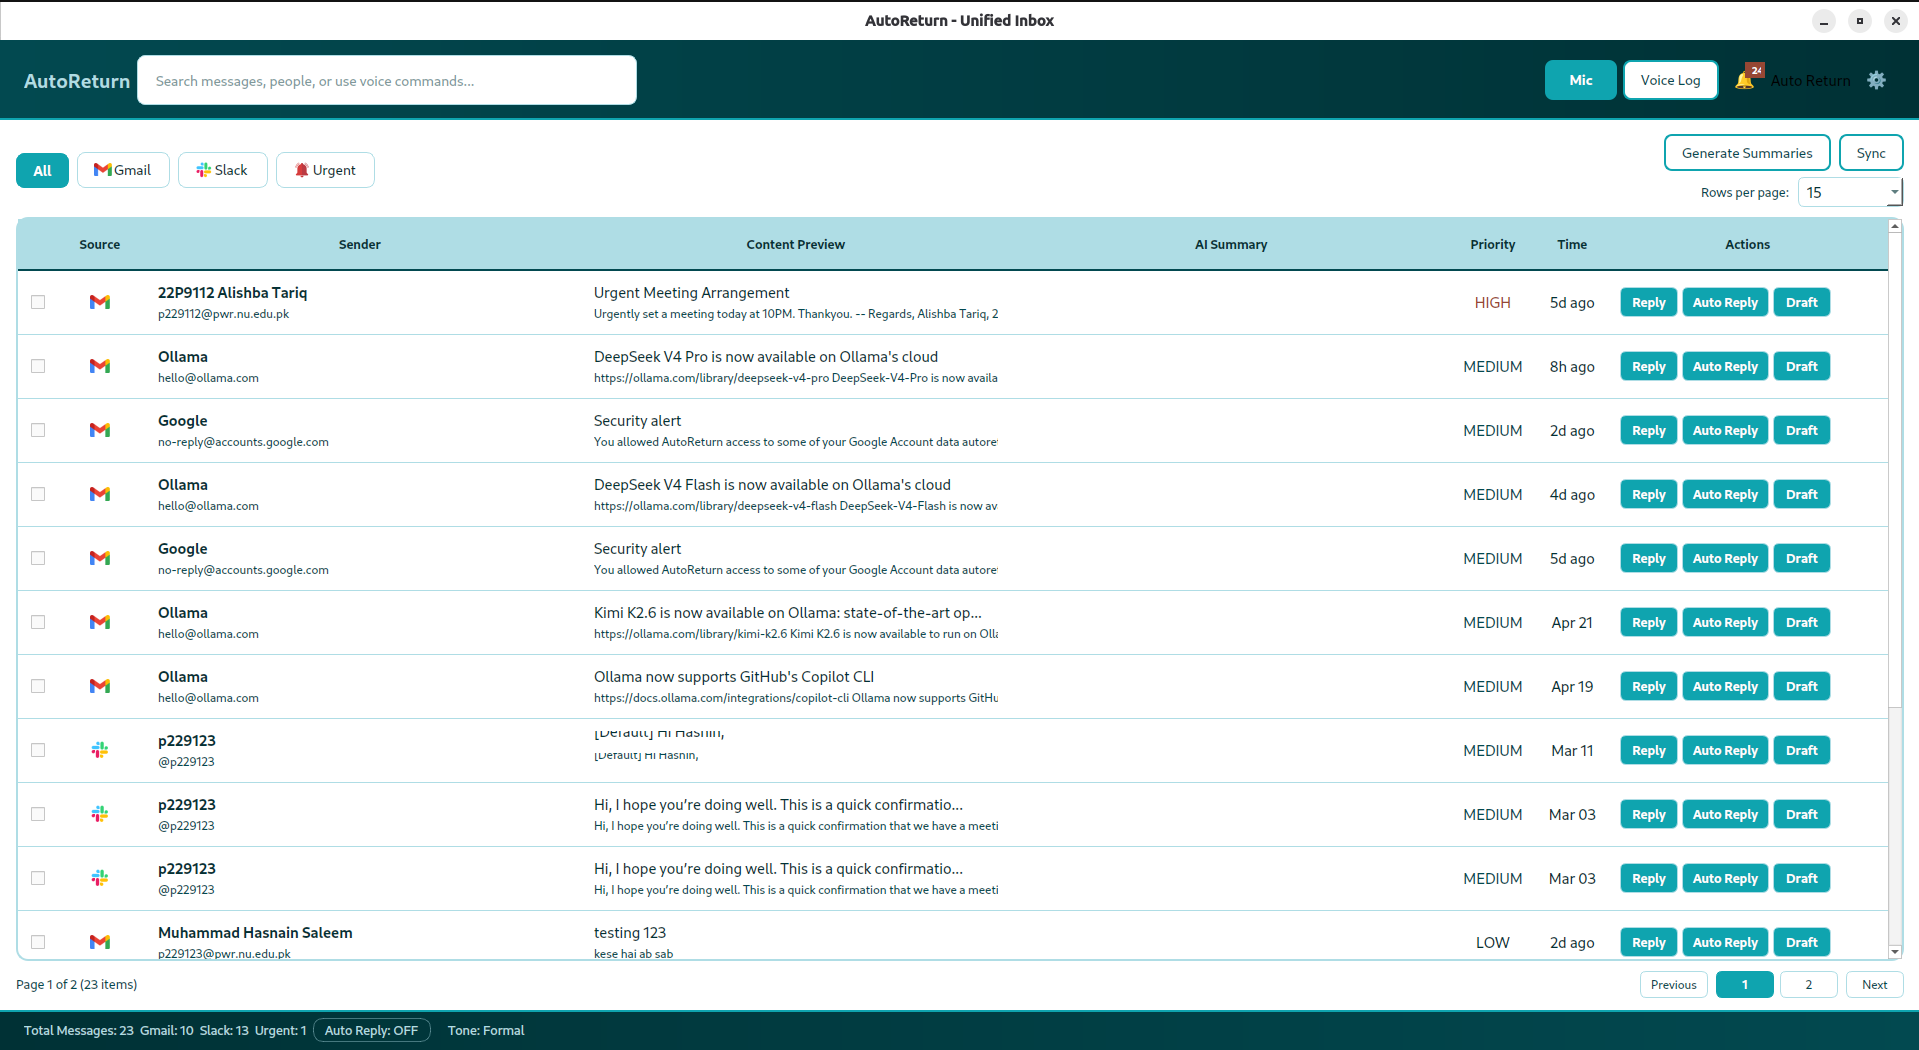
\includegraphics[width=0.98\linewidth,height=5.0cm,keepaspectratio]{Figures/Unified_Inbox_Dashboard.png}
        \caption{Unified Inbox Dashboard}
        \label{fig:ui_unified_inbox}
    \end{subfigure}

    \vspace{0.35em}

    \begin{subfigure}[t]{0.48\textwidth}
        \centering
        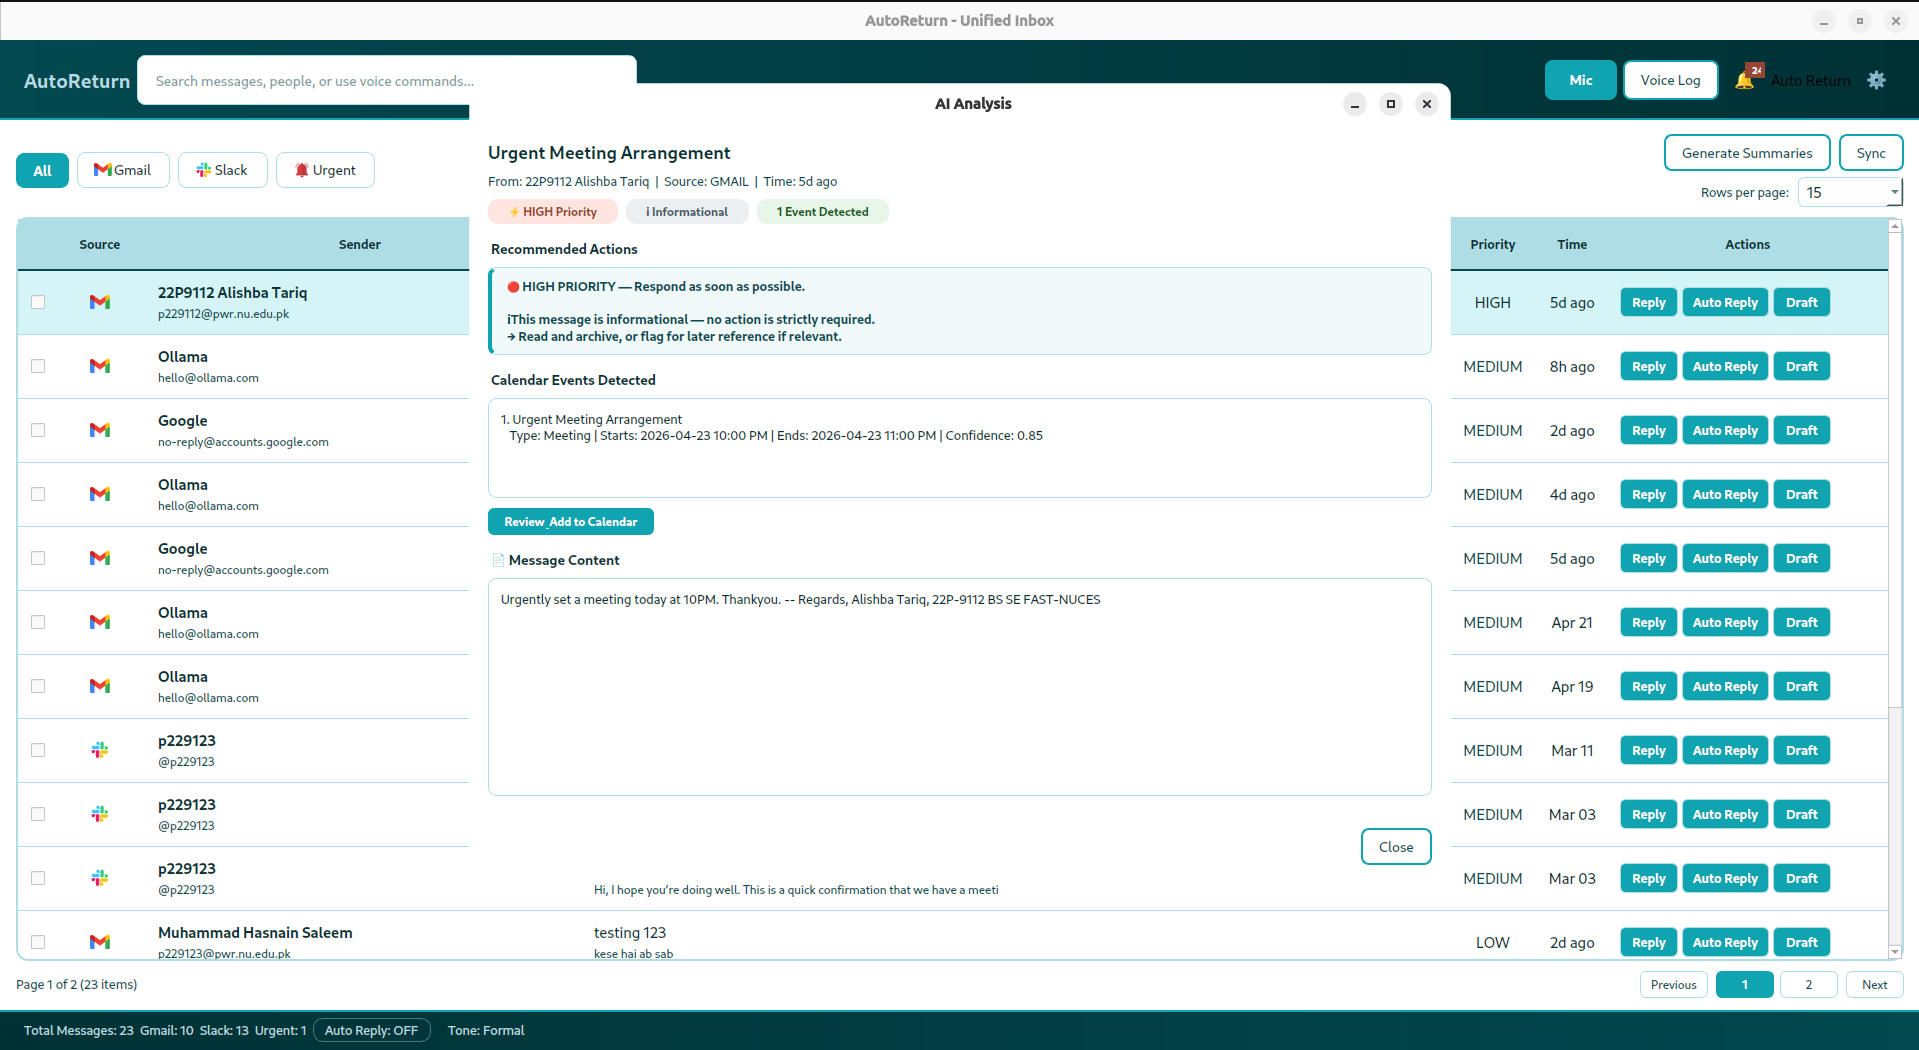
\includegraphics[width=0.98\linewidth,height=5.0cm,keepaspectratio]{Figures/Reply_Assistance.png}
        \caption{Reply Assistance}
        \label{fig:ui_reply_assistance}
    \end{subfigure}
    \hfill
    \begin{subfigure}[t]{0.48\textwidth}
        \centering
        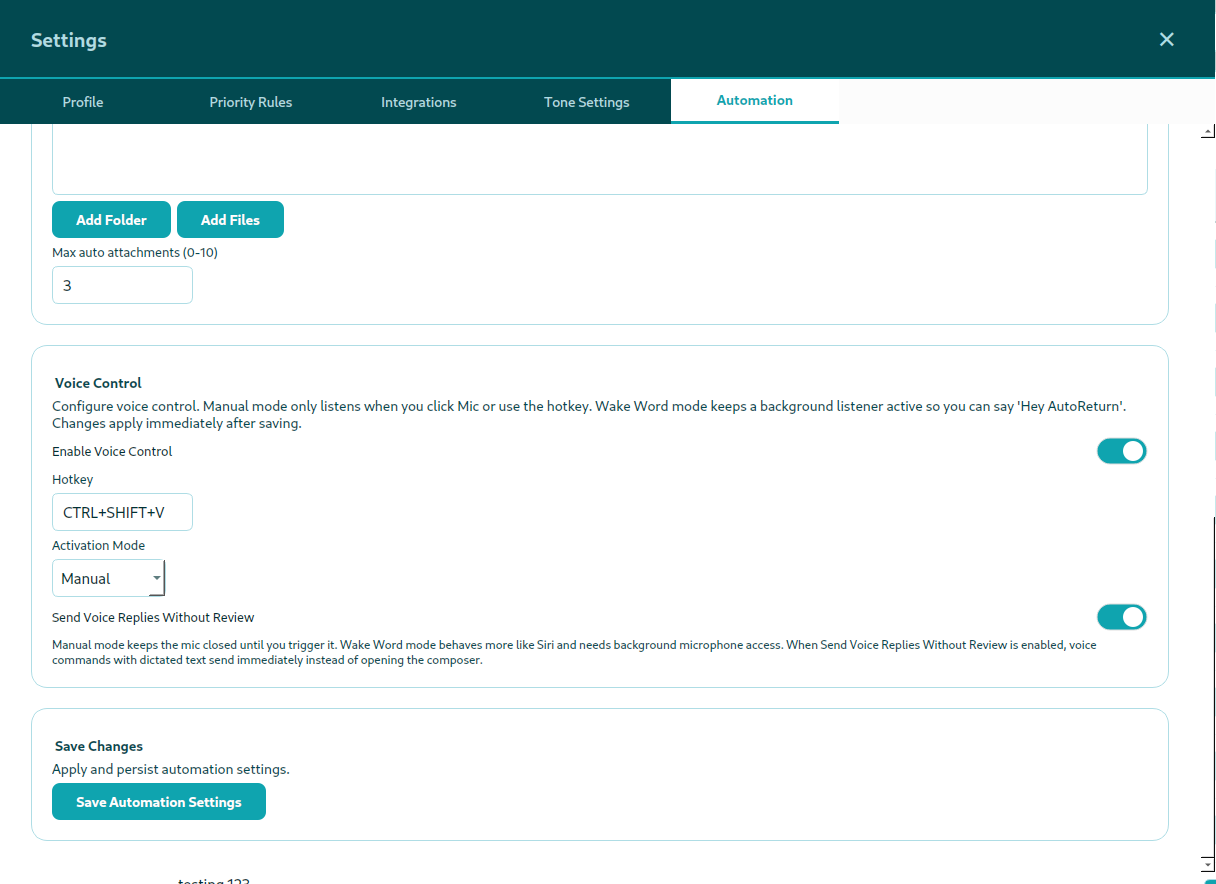
\includegraphics[width=0.98\linewidth,height=5.0cm,keepaspectratio]{Figures/Policy_Settings.png}
        \caption{Policy Settings}
        \label{fig:ui_policy_settings}
    \end{subfigure}
\caption{Primary AutoReturn Interface Screens}
\end{figure}

\begin{figure}[htbp]
    \centering
    \begin{subfigure}[t]{0.48\textwidth}
        \centering
        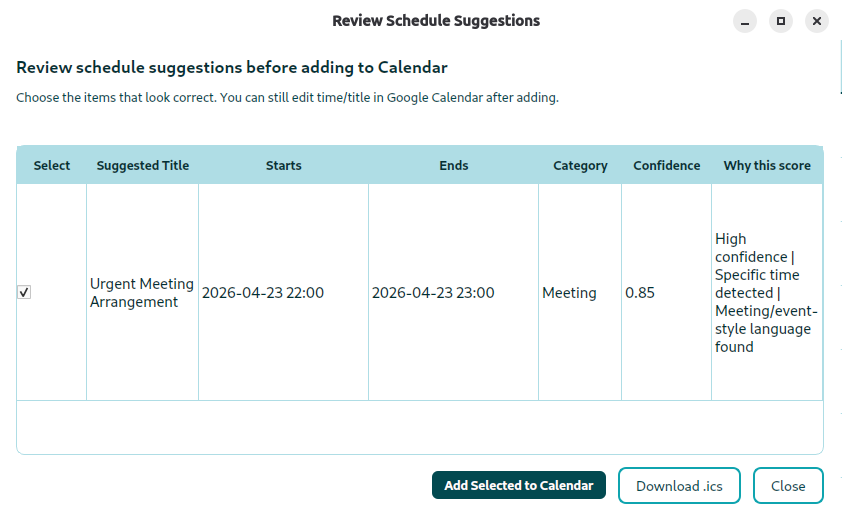
\includegraphics[width=0.98\linewidth,height=5.0cm,keepaspectratio]{Figures/Event_and_Calendar_Workflow.png}
        \caption{Event and Calendar Workflow}
        \label{fig:ui_event_workflow}
    \end{subfigure}
    \hfill
    \begin{subfigure}[t]{0.48\textwidth}
        \centering
        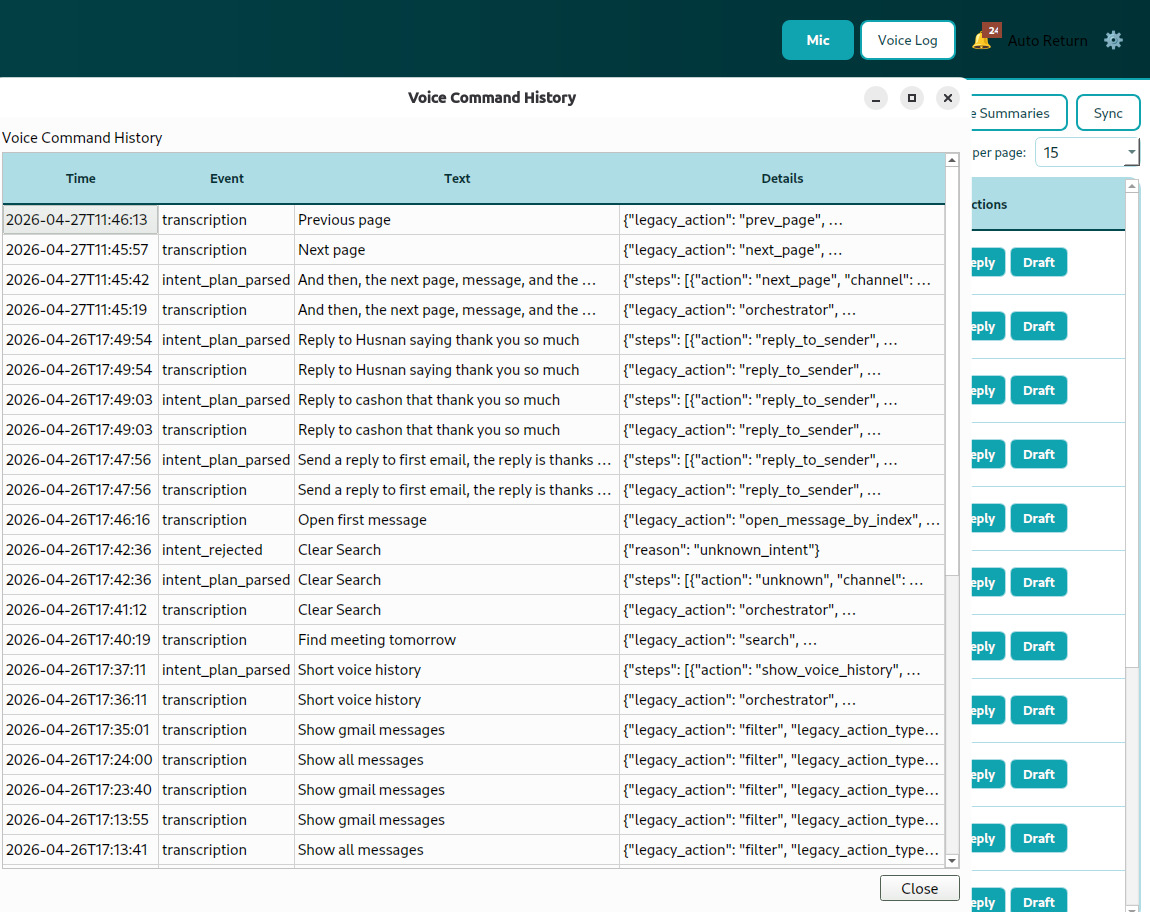
\includegraphics[width=0.98\linewidth,height=5.0cm,keepaspectratio]{Figures/Voice_Logs.png}
        \caption{Voice or Status Panel}
        \label{fig:ui_voice_status}
    \end{subfigure}
\caption{Additional AutoReturn Interface Screens}
\end{figure}

\section{Conclusion}
The final implementation demonstrates a working multi-service desktop prototype rather than an isolated proof of concept. Its strongest areas are platform integration, unified message handling, drafting support, priority assessment, and policy-aware automation. Features such as voice interaction and broader AI behavior are present but still less mature, so they are best understood as meaningful extensions of the core system rather than the primary basis of the project.

From an implementation perspective, the project shows that a modular orchestrator-agent design can support a realistic communication assistant without collapsing everything into a single opaque service layer. This provides a practical base for later refinement, broader testing, and more complete deployment support.

\chapter{Development Iterations}
\label{sec:iterations}

\section{Introduction}
This chapter presents the development progress of AutoReturn through the formal milestones used during the FYP lifecycle. The proposal, FYP-I mid, FYP-I final, FYP-II mid, and final thesis stage are treated as iteration checkpoints because each one captured a distinct state of scope, design, implementation, and evaluation.

Using these milestones as iterations makes the development story easier to trace in a way that matches the academic review process. Each stage therefore represents both a technical checkpoint and a documented refinement of project direction.

\section{Iteration Plan}
\noindent Table~\ref{tab:gantt_iteration_plan} reproduces the same phase plan used in the project presentations. It summarizes the planned progression from initial research to final testing and thesis completion.
\begin{table}[!htbp]
\centering
\small
\renewcommand{\arraystretch}{1.15}
\setlength{\tabcolsep}{5pt}
\begin{adjustbox}{width=\textwidth}
\begin{tabular}{|p{7.2cm}|p{2.3cm}|p{2.2cm}|p{2.2cm}|}
\hline
\textbf{Phase} & \textbf{Duration} & \textbf{Status} & \textbf{Semester} \\ \hline
Phase 1: Research \& Requirement Analysis & 0--3 Weeks & Completed & Semester 1 \\ \hline
Phase 2: System Design \& Architecture & 3--6 Weeks & Completed & Semester 1 \\ \hline
Phase 3: API Research \& Integration Testing & 6--12 Weeks & Completed & Semester 1 \\ \hline
Phase 4: Backend \& Core System Development & 12--18 Weeks & Completed & Semester 1,2 \\ \hline
Phase 5: Desktop App (Frontend) & 18--22 Weeks & Completed & Semester 1,2 \\ \hline
Phase 6: Smart Automation \& Features & 22--26 Weeks & Completed & Semester 1,2 \\ \hline
Phase 7: Testing, Evaluation \& Finalization & 26--28 Weeks & Completed & Semester 2 \\ \hline
\end{tabular}
\end{adjustbox}
\caption{Iteration Plan}
\label{tab:gantt_iteration_plan}
\end{table}

The value of this plan is not only chronological. It also shows how the project evolved from research and design into implementation, integration, evaluation, and final academic consolidation in a structured sequence.

\section{Iteration 1}
\subsection{Objectives}
The first iteration corresponded to the proposal stage. Its purpose was to validate the problem area, define the initial project direction, and determine whether operating-system-level workflow automation could be framed as a meaningful academic project.

\subsection{Major Deliverables}
The main deliverables of this stage were the initial project idea, the early problem statement, and the first scope assumptions.

\subsection{Iteration Outcome}
Review feedback during this stage showed that the original framing was too broad and not sufficiently grounded in a clear user workflow. As a result, the project direction was refined toward communication-centric workflow assistance. This outcome established the foundation for what later became AutoReturn.

\section{Iteration 2}
\subsection{Objectives}
The second iteration corresponds to the FYP-I mid evaluation. The main objective was to convert the corrected idea into a defendable system proposal supported by literature, investigation, modeling, and planning.

\subsection{Major Deliverables}
The major deliverables included the literature review, comparative investigation, initial use cases and UML artifacts, an early testing plan, and a clearer definition of the unified communication-workspace direction.

\subsection{Iteration Outcome}
This iteration produced the first academically structured version of the project. The system vision became clearer, but most of the work was still analytical and design-oriented. It also revealed that some early ideas, especially broad voice-first claims and feature breadth, would require later refinement.

\section{Iteration 3}
\subsection{Objectives}
The third iteration corresponds to the FYP-I final evaluation. The objective of this phase was to move from conceptual design toward implementation-driven development by formalizing the first core algorithms and workflow pipelines.

\subsection{Major Deliverables}
Deliverables in this stage included priority-classification logic, summary and draft-generation workflows, plain-text reply and task-classification pipelines, early Gmail integration work, and initial file-lookup and event-driven processing concepts.

\subsection{Iteration Outcome}
This stage marked the transition from proposal to implementation. The project now had identifiable backend logic and reproducible workflows, even though many features were still incomplete. It also clarified practical challenges such as Gmail automation limitations, dataset quality issues, and model-selection tradeoffs.

\section{Iteration 4}
\subsection{Objectives}
The fourth iteration corresponds to the FYP-II mid presentation. The objective of this phase was to expand the working prototype into a broader desktop system with stronger integration support, richer automation controls, and more formal testing evidence.

\subsection{Major Deliverables}
The main deliverables included the unified inbox and orchestrator-driven flow, Gmail and Slack agent integration, tone support and notification handling, auto-reply and DND behavior, calendar-related support, packaging and website material, and automated testing evidence with 111 tests.

\subsection{Iteration Outcome}
This iteration reflects the most visible growth in system maturity. The project evolved from isolated intelligent features into a more cohesive desktop workflow assistant. The presentation also documented important engineering improvements, including safer orchestrator behavior, better tone detection, improved attachment handling, and stronger cross-platform normalization.

\section{Iteration 5}
\subsection{Objectives}
The final iteration focused on consolidation and final thesis preparation. Its objective was to align the documentation, implementation, and evaluation with the actual final state of the project.

\subsection{Major Deliverables}
The major deliverables of this stage were final report refinement, chapter restructuring, removal of outdated claims, correction of testing and architecture descriptions, and alignment of modeling, implementation, and discussion with the completed prototype.

\subsection{Iteration Outcome}
This iteration transformed the project from a broad collection of implemented features into a more disciplined academic submission. The system was presented as a controlled prototype with verifiable scope, documented design decisions, and more defensible testing and discussion sections.

\chapter{Testing, Results, and Discussion}
\label{sec:testing}

\newcolumntype{Y}{>{\raggedright\arraybackslash}X}

\section{Testing Strategy}
The testing strategy was designed to cover both technical correctness and practical workflow behavior. Because AutoReturn coordinates multiple external services, automation rules, and model-assisted workflows, the evaluation had to combine reproducible backend checks with scenario-based validation of user-facing behavior.

\begin{itemize}
    \item Unit testing of individual agents (Gmail, Slack, Task Extraction)
    \item Integration testing of the unified inbox with model-assisted services
    \item End-to-end scenario testing for automated replies
    \item Performance-oriented checks for batch processing and core message workflows
    \item Manual validation of user-facing behaviors such as summaries, drafts, and settings
\end{itemize}

The formal automated suite was executed using a pytest-based workflow with trace-backed coverage reporting, which provided reproducible evidence for backend correctness and exercised the core automation paths of the system \cite{pytest2024,pythontrace2024}.

\section{Test Cases -- Part 1}
\begin{table}[!htbp]
\centering
\footnotesize
\renewcommand{\arraystretch}{1.15}
\setlength{\tabcolsep}{5pt}
\begin{adjustbox}{max width=\textwidth}
\begin{tabularx}{\textwidth}{|l|Y|Y|Y|Y|Y|Y|}
\hline
\textbf{ID} & \textbf{Scenario} & \textbf{Objective} & \textbf{Pre-conditions} & \textbf{Test Steps} & \textbf{Test Data} & \textbf{Expected Result} \\ \hline
TC\_INT\_01 & Verify multi-app integration (Slack + Gmail) & Ensure APIs connect successfully & Valid tokens & Connect apps and fetch messages & OAuth keys & Unified inbox retrieved \\ \hline
TC\_AUTO\_01 & Auto email summarization & Verify NLP summaries & Gmail linked & Run summarization & Sample emails & Concise summaries shown \\ \hline
TC\_TASK\_01 & Actionable information extraction & Ensure events or follow-up items are identified & Slack + Gmail active & Run extractor & Message text & Structured extracted output generated \\ \hline
TC\_NOTIF\_01 & Configurable alerts & Validate custom notifications & Event rule set & Trigger alert condition & "Interview call" email & Notification triggered \\ \hline
TC\_DASH\_01 & Unified inbox display & Verify dashboard merges notifications & Apps linked & Open dashboard & Message events & Combined view accurate \\ \hline
TC\_STATUS\_01 & Voice command parsing & Check that supported voice input is transcribed and routed correctly & Mic active & Speak a supported command & Voice input & Command mapped to the expected UI action or workflow \\ \hline
\end{tabularx}
\end{adjustbox}
\caption{Test Cases – Integration and Automation}
\end{table}
\FloatBarrier

These cases emphasize the main communication workflows that define AutoReturn’s practical value, especially integration, summarization, extraction, notifications, and dashboard behavior. They were selected because they represent the most visible user-facing paths in the implemented system.

\section{Test Cases -- Part 2}
\begin{table}[!htbp]
\centering
\footnotesize
\renewcommand{\arraystretch}{1.15}
\setlength{\tabcolsep}{5pt}
\begin{adjustbox}{max width=\textwidth}
\begin{tabularx}{\textwidth}{|l|Y|Y|Y|Y|Y|Y|}
\hline
\textbf{ID} & \textbf{Scenario} & \textbf{Objective} & \textbf{Pre-conditions} & \textbf{Test Steps} & \textbf{Test Data} & \textbf{Expected Result} \\ \hline
TC\_REMIND\_01 & Follow-up reminder & Ensure reminders trigger correctly & Gmail + Slack active & Set reminder, simulate delay & Reminder = 3h & Alert generated \\ \hline
TC\_SENTI\_01 & Sentiment analysis & Validate emotion or urgency detection & NLP model active & Analyze strong message tone & "URGENT! Project failed" & Marked as urgent \\ \hline
TC\_LOG\_01 & Audit trail logging & Ensure action logs recorded & Admin access & Perform actions, open log & Log entries & Accurate timestamps \\ \hline
TC\_ACCESS\_01 & Access revocation & Check permission removal & Active session & Revoke Gmail access & Gmail token & Access denied message \\ \hline
TC\_OFFLINE\_01 & Offline functionality & Validate limited offline support & Cached data available & Disconnect, run summary & Cached threads & Summary shown locally \\ \hline
TC\_SECURITY\_01 & Token encryption & Verify secure local storage & Tokens issued & Inspect encrypted store & Access tokens & Encrypted securely \\ \hline
\end{tabularx}
\end{adjustbox}
\caption{Test Cases – Notifications, Security, and Reliability}
\end{table}
\FloatBarrier

The second group complements the first by covering reminders, logging, revocation, offline behavior, and credential protection. Together, both test-case sets provide a broader view of the system than feature validation alone.

\section{Testing Outcomes}
Testing confirmed that the core implementation is functional across the main backend workflows, especially for integration, summarization, drafting, classification, and automation logic. The results are encouraging, but they should be interpreted carefully: the current test suite provides meaningful technical evidence, yet it does not by itself prove full production readiness or broad user validation.

Based on the documented successful full-suite run dated 2026-03-08, the system achieved the following results:
\begin{table}[!htbp]
\centering
\small
\renewcommand{\arraystretch}{1.15}
\setlength{\tabcolsep}{5pt}
\begin{tabular}{|l|c|c|c|}
\hline
\textbf{Test Category} & \textbf{Total Tests} & \textbf{Failures} & \textbf{Status} \\ \hline
Formal automated suite & 111 & 0 & Successful \\ \hline
\end{tabular}
\caption{Test Execution Results}
\end{table}

\begin{table}[!htbp]
\centering
\small
\renewcommand{\arraystretch}{1.15}
\setlength{\tabcolsep}{6pt}
\begin{tabular}{|>{\raggedright\arraybackslash}p{5.8cm}|>{\centering\arraybackslash}p{4.8cm}|}
\hline
\textbf{Metric} & \textbf{Value} \\ \hline
Total Tests Executed & 111 \\
Test Failures & 0 \\
Successful Execution & 111 / 111 tests completed \\
Code Coverage & 30.47\% \\
Test Duration & 33.6 seconds \\
Execution Platform & macOS 12.7.6 (x86\_64) \\
\hline
\end{tabular}
\caption{Comprehensive Test Metrics}
\end{table}

Overall code coverage reached 30.47\% across 7,529 executable statements. The formal suite directly covered 2,294 statements while exercising the core integration, orchestration, summarization, drafting, and policy-handling paths. Coverage was strongest in backend workflow logic, which is appropriate because the most critical technical risk in this project lay in multi-service coordination rather than purely visual interface rendering.

\section{Performance Metrics}
\begin{table}[!htbp]
\centering
\small
\renewcommand{\arraystretch}{1.15}
\setlength{\tabcolsep}{6pt}
\begin{tabular}{|>{\raggedright\arraybackslash}p{6.0cm}|>{\centering\arraybackslash}p{4.6cm}|}
\hline
\textbf{Performance Indicator} & \textbf{Observed Result} \\ \hline
Full automated suite duration & 33.6 seconds \\ \hline
Tests executed in one run & 111 \\ \hline
Average throughput & 3.31 tests/second \\ \hline
Run completion status & Successful \\ \hline
Observed workflow responsiveness & Stable for prototype-scale inbox, drafting, and settings workflows \\ \hline
\end{tabular}
\caption{Observed Performance Indicators}
\end{table}

The measured full-suite execution time shows that the implemented backend workflows can be exercised within well under one minute on a standard desktop environment. In practical use, summarization, drafting, classification, and settings-related actions remained responsive enough for interactive prototype operation. These measurements do not replace a full production benchmark program, but they provide concrete evidence that the system performs acceptably for the scope of the final project.

\section{Key Technical Challenges Identified}
\begin{table}[!htbp]
\centering
\small
\renewcommand{\arraystretch}{1.15}
\setlength{\tabcolsep}{5pt}
\begin{adjustbox}{width=\textwidth}
\begin{tabular}{|>{\raggedright\arraybackslash}p{3.3cm}|>{\raggedright\arraybackslash}p{5.2cm}|>{\raggedright\arraybackslash}p{6cm}|}
\hline
\textbf{Challenge Area} & \textbf{Observed Issue} & \textbf{Project Response} \\ \hline
Model workflow optimization & Runtime choice, response delay, and context-length handling affected summary, draft, and extraction consistency. & The final system used configurable model routing, message-cleaning steps, and more conservative prompt flow so that intelligent services remained practical for desktop use. \\ \hline
System integration & Gmail, Slack, and shared backend services exposed different message structures, credential states, and synchronization conditions. & The orchestrator-agent design normalized cross-platform data and isolated integration responsibilities so downstream automation could operate on a shared message model. \\ \hline
Privacy and security & Local credential handling, automation safety, and user trust were critical because the application processes communication data. & Token protection, review-first behavior, allowlists, DND controls, and explicit policy checks were used to keep automation controlled and safer by default. \\ \hline
\end{tabular}
\end{adjustbox}
\caption{Key Technical Challenges Identified During Testing}
\end{table}

These challenge areas are especially relevant because they connect testing outcomes with design priorities. They also show that the final prototype was shaped as much by risk management and reliability concerns as by feature expansion.

\section{Discussion}
The testing phase revealed several important insights about system maturity. Core backend workflows are in place and technically demonstrable, but the evidence also shows that the project is still in a prototype stage where further stabilization, broader coverage, and fuller user-facing validation are needed.

\textbf{Strengths.} The strongest outcome of testing is that the system demonstrates robust Gmail and Slack integration together with working automation paths for summarization, drafting, classification, and event-related workflows. The project also provides meaningful automated evidence for backend logic and preserves a clear architecture for continued refinement.

\textbf{Areas for Improvement.} The next improvement priorities are to increase automated coverage across additional modules, expand performance measurement beyond basic execution results, and complete and validate voice-related workflows more thoroughly.

\section{Conclusion}
The testing and evaluation phase shows that AutoReturn satisfies a substantial portion of its core technical objectives, especially in integration, orchestration, and intelligent workflow support. However, the results should be read as evidence of a capable academic prototype rather than a fully polished production system. The most important next steps are broader verification, deeper performance evaluation, and further refinement of partially mature features.

Even so, the current evidence is strong enough to support the main academic claim of the project: that a unified, AI-assisted communication workspace can be built as a controlled desktop prototype with meaningful automation and measurable backend validation.

\chapter{Project Management and Deployment Considerations}
\label{sec:project_management}

\section{Project Timeline}
The timeline in Table~\ref{tab:project_timeline} follows the same phase schedule used in the iteration chapter so that planning evidence remains consistent across the report.
\begin{table}[!htbp]
\centering
\small
\renewcommand{\arraystretch}{1.15}
\setlength{\tabcolsep}{5pt}
\begin{adjustbox}{width=\textwidth}
\begin{tabular}{|>{\raggedright\arraybackslash}p{8cm}|>{\raggedright\arraybackslash}p{2.5cm}|>{\raggedright\arraybackslash}p{2.5cm}|>{\raggedright\arraybackslash}p{2.5cm}|}
\hline
\textbf{Phase} & \textbf{Duration} & \textbf{Status} & \textbf{Semester} \\ \hline
Phase 1: Research \& Requirement Analysis & 0--3 Weeks & Completed & Semester 1 \\ \hline
Phase 2: System Design \& Architecture & 3--6 Weeks & Completed & Semester 1 \\ \hline
Phase 3: API Research \& Integration Testing & 6--12 Weeks & Completed & Semester 1 \\ \hline
Phase 4: Backend \& Core System Development & 12--18 Weeks & Completed & Semester 1,2 \\ \hline
Phase 5: Desktop App (Frontend) & 18--22 Weeks & Completed & Semester 1,2 \\ \hline
Phase 6: Smart Automation \& Features & 22--26 Weeks & Completed & Semester 1,2 \\ \hline
Phase 7: Testing, Evaluation \& Finalization & 26--28 Weeks & Completed & Semester 2 \\ \hline
\end{tabular}
\end{adjustbox}
\caption{Project Timeline}
\label{tab:project_timeline}
\end{table}
\FloatBarrier

This timeline also shows that implementation, integration, testing, and reporting were handled as coordinated phases rather than as isolated late-stage tasks. That structure helped the team keep the academic deliverables aligned with the actual technical progress of the project.

\section{Risk Management}
\begin{table}[!htbp]
\centering
\small
\renewcommand{\arraystretch}{1.15}
\setlength{\tabcolsep}{5pt}
\begin{adjustbox}{width=\textwidth}
\begin{tabular}{|>{\raggedright\arraybackslash}p{2cm}|>{\raggedright\arraybackslash}p{5cm}|>{\raggedright\arraybackslash}p{6cm}|}
\hline
\textbf{Risk ID} & \textbf{Risk} & \textbf{Mitigation} \\ \hline
R1 & Authentication expiry and integration instability & Token refresh handling, safer local storage, and more controlled service logic. \\ \hline
R2 & Voice interaction inconsistency & Confidence-based fallback and continued reliance on manual interaction for less mature scenarios. \\ \hline
R3 & Integration failure across services & Retry logic, logging, isolation of service responsibilities, and staged testing. \\ \hline
R4 & LLM output inconsistency & Prompt refinement, constrained output handling, and validation in downstream workflows. \\ \hline
R5 & Cross-platform interface issues & Use of PySide6 and repeated interface refinement for more consistent behavior. \\ \hline
\end{tabular}
\end{adjustbox}
\caption{Key Project Risks and Mitigation Measures}
\end{table}

These risks were tracked throughout development because the project depended on multiple external services, user-facing automation, and model-assisted behavior. As a result, mitigation planning was treated as a continuing engineering activity rather than a one-time management formality.

\section{Team Work Distribution}
All three members contributed throughout requirements analysis, implementation, testing, presentations, and report preparation. Their primary ownership areas are summarized below, but the project was completed through continuous joint effort rather than isolated task silos.

\begin{table}[!htbp]
\centering
\footnotesize
\renewcommand{\arraystretch}{1.15}
\setlength{\tabcolsep}{5pt}
\begin{adjustbox}{width=\textwidth}
\begin{tabular}{|>{\raggedright\arraybackslash}p{3.0cm}|>{\raggedright\arraybackslash}p{6.0cm}|>{\raggedright\arraybackslash}p{5.2cm}|}
\hline
\textbf{Member} & \textbf{Primary Ownership and Implemented Features} & \textbf{Shared Contribution Areas} \\ \hline
Muhammad Hasnain Saleem & Voice-enabled actions, wake-word activation, calendar feature, priority handling, and message-data workflows including synchronized processing pathways used by the unified inbox and downstream automation features. & Testing, presentations, report preparation, refinement of implemented workflows, and final system consolidation. \\ \hline
Kashan Saeed & Core framework, orchestration logic, AI-service integration, orchestrator, unified inbox backbone, email/message summary, draft generation, plain-text response flow, task classification, task extraction, CI/CD support, and core deployment packaging direction. & Architecture refinement, testing, presentations, documentation, and stabilization of the final desktop prototype. \\ \hline
Alishba Tariq & Tone preference, Gmail agent, Slack agent, event-driven file lookup, search, desktop and pop-up notifications, sender statistics, website and deployment work, DND, auto-reply behavior, and supporting backend integrations for user-facing workflows. & Interface refinement, testing, presentations, report structuring, documentation, and final evaluation alignment. \\ \hline
\end{tabular}
\end{adjustbox}
\caption{Team Work Distribution}
\end{table}

\section{Change Management}
The project evolved from a broad operating-system automation idea into a communication-centered assistant focused on Gmail and Slack. During FYP-II, the implementation matured into a native PySide6 desktop application with orchestrator-agent coordination, unified message handling, policy-based automation, event extraction, and attachment-control workflows. Voice support was retained as a supporting feature, but its scope was narrowed so the final system remained aligned with the most stable and testable workflows.

This process of change was important because it prevented the project from remaining too broad or speculative. Instead, the final report and prototype now reflect a more disciplined scope that matches what was actually implemented and validated.

\section{Project Closure}
The project closure produced a working desktop prototype, documented source code, test evidence, presentation material, and the final thesis report. The resulting system remains an academic prototype, but it establishes a stable base for further packaging, broader platform testing, and continued refinement of communication automation features.

In that sense, closure in this project does not mean technical finality. It means that the work has reached a coherent and defensible stopping point for academic evaluation, while still leaving room for future extension beyond the FYP timeline.

\chapter{User Manual}
\label{sec:user_manual}

\section{Introduction}
This user manual provides a practical guide for operating AutoReturn as a unified Gmail- and Slack-based communication workspace. It explains how the application is started, configured, and used in day-to-day workflows.

The focus of this chapter is on the user-facing flow of the system rather than on internal architecture. For that reason, the following sections describe the sequence of use from sign-in and account connection to message handling, settings control, and routine troubleshooting.

\section{Getting Started}
To begin using AutoReturn, the user launches the desktop application, signs in, and connects the supported Gmail and Slack accounts. Once the accounts are active, the main dashboard becomes available for message review, summaries, reply assistance, event inspection, and automation settings.

\begin{enumerate}
    \item Launch AutoReturn and sign in through the authentication interface.
    \item Connect the available Gmail and Slack accounts.
    \item Open the unified inbox dashboard to review synchronized messages.
    \item Select a message to inspect details, summaries, and reply suggestions.
    \item Configure automation policies, quiet rules, or reply preferences from the settings area.
    \item Review event extraction, attachment suggestions, or calendar export options when relevant.
\end{enumerate}

\section{User Interface Guide}
The login and account-connection screens are used to authenticate the user and activate the supported platforms. After authentication, the unified inbox dashboard becomes the central workspace for reviewing Gmail and Slack content, summaries, priority cues, and notification items. Selecting a message opens the detail view, where the user can inspect the content, generate a summary, review a draft reply, or choose a controlled response mode.

The settings area is used to configure quiet hours, allowlists, DND rules, and reply behavior. Event-related workflows are also available when messages contain scheduling details, allowing the user to inspect extracted information and export an ICS file when relevant. Together, these screens represent the main operational path through the application.

\section{Features and Functionality}
AutoReturn combines several user-facing capabilities within one desktop workflow. The main system functions are summarized below:

\begin{enumerate}
    \item \textbf{Unified Communication Workspace:} Gmail and Slack messages are brought into a shared inbox for centralized review.
    \item \textbf{Message Summarization:} Supported messages can be summarized to reduce reading effort and highlight key points quickly.
    \item \textbf{Draft Generation and Reply Assistance:} The system can prepare contextual reply drafts and tone-adjusted suggestions for user review.
    \item \textbf{Priority Classification:} Messages are scored using keyword, deadline, and sender signals to estimate urgency.
    \item \textbf{Automation Policy Control:} Draft-only, plain-reply, auto-reply, allowlist, and DND behavior can be configured by the user.
    \item \textbf{Event Extraction and Calendar Export:} Time-related information can be identified and prepared for calendar-oriented workflows.
    \item \textbf{Voice-Supported Interaction:} The application provides partial support for push-to-talk capture, transcription, and supported command routing.
    \item \textbf{Attachment Assistance:} File requests can be matched against approved locations, with ambiguous cases blocked for manual confirmation.
\end{enumerate}

\section{Frequently Asked Questions (FAQs)}
\begin{enumerate}
    \item \textbf{How do I sign in and connect my accounts?} \\
    Open AutoReturn, complete the authentication step, and connect the available Gmail and Slack accounts from the connection screen. Once the accounts are linked, the system can retrieve communication data and enable the unified workspace.

    \item \textbf{Where can I see all incoming communication?} \\
    All synchronized Gmail and Slack content is shown in the unified inbox dashboard. This is the main area for reviewing recent items, alerts, and prioritized communication.

    \item \textbf{How do I generate a summary or reply draft?} \\
    Select a message from the dashboard and open its detail view. From there, the available assistance features can generate a summary, prepare a draft reply, and present tone-aware suggestions for review.

    \item \textbf{How do I control automation behavior?} \\
    Automation settings are managed through the policy and settings area. Here, the user can configure DND, allowlists, draft-only behavior, plain replies, and other rule-based controls that determine how the system handles communication.
\end{enumerate}

\chapter{Conclusions and Future Work}
\label{sec:conclusions}

\section{Conclusion}
This project set out to address the fragmentation of modern communication workflows by designing an intelligent desktop system that can unify Gmail and Slack interactions and support them with automation. The final implementation shows that this objective is achievable to a meaningful extent through a modular orchestrator-agent architecture, user-controlled model integration, policy-based automation, and a native desktop interface.

The completed system provides several practical capabilities: unified message handling, draft generation, summarization, tone-aware assistance, priority classification, event extraction, attachment resolution support, and configurable response behavior. These features show that AutoReturn is more than a conceptual integration layer. It is a functioning productivity prototype that combines multiple communication-support workflows within one environment.

The project also made clear that intelligent communication automation requires careful boundaries. Model output must be constrained, automation rules must remain transparent, and ambiguous cases must fall back to explicit user control. This insight shaped the priority engine, policy settings, and ambiguity-blocking logic. As a result, the project contributes not only an implementation, but also a practical lesson in balancing assistance with controllability.

\textbf{Key Outcomes.}
\begin{itemize}
    \item A native desktop application was developed to consolidate Gmail- and Slack-based workflows.
    \item An orchestrator-agent design was used to structure integrations and keep the system extensible.
    \item AI-assisted features were implemented for summarization, drafting, extraction, classification, and tone support.
    \item Policy-based automation was introduced to support draft-only, plain-reply, auto-reply, DND, and allowlist behavior.
    \item The project established a foundation for future expansion without requiring the current report to claim fully finished enterprise readiness.
\end{itemize}

These outcomes matter because they demonstrate that the project advanced beyond conceptual integration and into a functioning prototype with meaningful technical depth. They also show that AutoReturn contributes both an implemented system and a reusable architectural direction for future refinement.

\section{Limitations}
Despite its strengths, AutoReturn remains an academic prototype with several limitations. Integration support is still focused on a small number of platforms. Voice functionality, while more developed than in the earlier concept phase, is not yet a complete conversational subsystem.

Performance and behavior may vary depending on model setup, device capabilities, and external API conditions. In addition, some advanced scenarios still require manual confirmation because full automation would introduce unacceptable ambiguity or trust risk.

\section{Future Work}
Future work should concentrate on strengthening depth rather than simply adding breadth. The most valuable next steps are:
\begin{itemize}
    \item Expanding platform integrations only after the current Gmail and Slack workflows are further stabilized.
    \item Improving packaging and deployment for easier installation across supported operating systems.
    \item Refining voice interaction so that command capture, transcription, and workflow execution operate more reliably and consistently.
    \item Strengthening evaluation with broader testing, better performance profiling, and more structured user feedback collection.
    \item Improving explainability so users can better understand why the system produced a given priority, summary, or automation decision.
    \item Extending policy controls and permission boundaries for safer automation in more sensitive communication scenarios.
\end{itemize}

These next steps are deliberately focused on maturity and reliability rather than on feature inflation. That direction is consistent with the overall lesson of the project: controlled refinement is more valuable than unchecked expansion in communication-centered automation systems.

Overall, AutoReturn demonstrates that a privacy-aware, AI-assisted communication workspace can be built as a coherent desktop system rather than as a loose collection of wrappers and cloud automations. The project does not solve every challenge of intelligent workflow automation, but it establishes a strong technical and architectural base for further development.


% -------------------------
% REFERENCES AND APPENDIX
% Adds the manual references list and supplementary links.
\addcontentsline{toc}{chapter}{References}
\begingroup
\small
\sloppy
\raggedright
\begin{thebibliography}{99}

\bibitem{bentahar2005}
J. Bentahar, \emph{A Pragmatic and Semantic Unified Framework for Agent Communication}. Université Laval, Doctoral Thesis, 2005.

\bibitem{cao2024}
J. Cao, ``Deploying Large Language Models as Agents,'' MIT CSAIL, 2024.

\bibitem{kumar2015}
G. V. Kumar and P. Jayanthi, ``Real-Time Text and Speech Recognition System,'' \emph{JNAO Journal}, 2015.

\bibitem{spacy2024}
Explosion AI, ``spaCy Documentation,'' 2024. Available: \url{https://spacy.io/}. Accessed: Jan. 12, 2026.

\bibitem{gmail2023}
Google, ``Gmail API Documentation,'' 2023. Available: \url{https://developers.google.com/gmail/api}. Accessed: Dec. 18, 2025.

\bibitem{slack2023}
Slack, ``Slack API Documentation,'' 2023. Available: \url{https://api.slack.com/}. Accessed: Dec. 21, 2025.

\bibitem{ferdium2024}
Ferdium Community, ``Ferdium App -- GitHub Repository,'' 2024. Available: \url{https://github.com/ferdium/ferdium-app}. Accessed: Oct. 10, 2025.

\bibitem{wavebox2024}
Wavebox Team, ``Wavebox -- Official Website,'' 2024. Available: \url{https://wavebox.io/}. Accessed: Oct. 12, 2025.

\bibitem{beeper2024}
Beeper Team, ``Beeper -- Product Information,'' 2024. Available: \url{https://www.beeper.com/}. Accessed: Oct. 14, 2025.

\bibitem{shift2024}
Shift Team, ``Shift -- Product Overview,'' 2024. Available: \url{https://shift.com/}. Accessed: Oct. 15, 2025.

\bibitem{superhuman2024}
Superhuman Team, ``Superhuman -- Product Overview,'' 2024. Available: \url{https://superhuman.com/}. Accessed: Oct. 17, 2025.

\bibitem{front2024}
Front Team, ``Front -- Shared Inbox and Team Communication Platform,'' 2024. Available: \url{https://front.com/}. Accessed: Oct. 20, 2025.

\bibitem{respond2024}
Respond.io Team, ``Respond.io -- Product Overview,'' 2024. Available: \url{https://respond.io/}. Accessed: Oct. 22, 2025.

\bibitem{technode2022}
TechNode Global, ``Respond.io Raises \$7M Funding Led by Headline Asia,'' 2022. Available: \url{https://technode.global/2022/09/13/respond-io-raises-7m-funding-led-by-headline-asia/}. Accessed: Oct. 24, 2025.

\bibitem{chatwoot2024}
Chatwoot Team, ``Chatwoot -- Official Website,'' 2024. Available: \url{https://www.chatwoot.com/}. Accessed: Oct. 25, 2025.

\bibitem{ollama2024}
Ollama Team, ``Ollama Documentation,'' 2024. Available: \url{https://ollama.com/}. Accessed: Jan. 08, 2026.

\bibitem{pyside2024}
Qt for Python Team, ``PySide6 Documentation,'' 2024. Available: \url{https://doc.qt.io/qtforpython-6/}. Accessed: Dec. 10, 2025.

\bibitem{supabase2024}
Supabase Team, ``Supabase Documentation,'' 2024. Available: \url{https://supabase.com/docs}. Accessed: Feb. 05, 2026.

\bibitem{whisper2023}
OpenAI, ``Whisper Speech Recognition Repository,'' 2023. Available: \url{https://github.com/openai/whisper}. Accessed: Feb. 18, 2026.

\bibitem{pytest2024}
pytest Development Team, ``pytest Documentation,'' 2024. Available: \url{https://docs.pytest.org/}. Accessed: Mar. 03, 2026.

\bibitem{pythontrace2024}
Python Software Foundation, ``Python trace Module Documentation,'' 2024. Available: \url{https://docs.python.org/3/library/trace.html}. Accessed: Mar. 05, 2026.

\bibitem{rfc5545}
B. Desruisseaux, ``Internet Calendaring and Scheduling Core Object Specification (iCalendar),'' RFC 5545, Internet Engineering Task Force, 2009.

\end{thebibliography}
\endgroup


\appendix
\chapter{Supplementary Material}
\label{app:supplementary_material}

This appendix provides the primary supplementary resources associated with AutoReturn. These materials support reproducibility, external review, and demonstration of the final project beyond the printed thesis document.

\section{Project Repository}
The source code, implementation history, and development artifacts are available in the official project repository:

\noindent
\url{https://github.com/hasnainsaleem18/AutoReturn}

The repository contains the desktop application codebase, backend services, integration logic, testing assets, and related project files used during development and evaluation.

\section{Project Website}
The project website presents the public-facing overview of AutoReturn, including product context, summary material, and supporting presentation content:

\noindent
\url{https://autoreturn.vercel.app/}

Together, these resources complement the thesis by providing direct access to the implemented system and its supporting material in a compact, non-duplicative form.


\end{document}
